%!TEX root = ../report.tex

\begin{document}
    \chapter{Evaluation and Results}
    
    In this section, we will report quantitative and qualitative analysis of the results obtained from 2D Lane Detection, and binary lane segmentation, followed by the resulting 3D Lane detection approaches discussed in sections 4.2.3 and 4.2.6. Moreover, we will discuss in detail the current status of the proposed dual-stage semi-local 3D lane detector. 
    
    \section{2D Lane Detection}
    As in our proposed approach, we have adopted the dual-stage way of predicting 3D lane curves inspired by \cite{guo2020gen}, where the first stage is binary lane segmentation followed by a 3D lane detector. Considering the uniqueness of the task of 2D lane detection as we need to capture rich vision cues from the environment, we explored approaches like SCNN \cite{pan2018SCNN}, Ufld \cite{DBLP:journals/corr/abs-2004-11757}, CondLaneNet \cite{DBLP:journals/corr/abs-2105-05003}, RESA \cite{DBLP:journals/corr/abs-2008-13719},  LaneATT \cite{https://doi.org/10.48550/arxiv.2010.12035}, Enet-SAD \cite{DBLP:journals/corr/abs-1908-00821} which are performing the task of 2D Lane Detection. Though this work is mainly focused on detecting 2D lane lines via the means of segmentation, we have carried out a comparative evaluation of the above-mentioned approaches which will form the base of experimentation for binary lane segmentation. All the above-mentioned approaches were trained on  CULane \cite{pan2018SCNN} and TuSimple \cite{Tusimple}. Our motive for this evaluation was to obtain the best-performing segmentation-based 2D lane detection architecture. We have evaluated these approaches using pre-trained models on the above-mentioned datasets. The evaluation metrics used are $F1$ score and accuracy: 
    
    \begin{equation}
        F1 = \frac{2*precision * recall}{precision + recall}
    \end{equation}
    
where, $precision = \frac{TP}{TP + FP}$ and $recall = \frac{TP}{TP + FN}$. Like in the case of the CULane \cite{pan2018SCNN} dataset each lane is composed of 30-pixel width and IoU(Intersection Over Union) is calculated between the predictions and ground-truth. If $IoU > 0.5$, it is treated as TP. 
For TuSimple dataset accuracy is used as an official metric to evaluate an approach which can be defined as, $accuracy =\frac{\sum_{clip} C_{clip}}{ \sum_{clip} C_{clip}}$. Where $S_{clip}$ represents the total number of points in the clip and $C_{clip}$ is the total number of points predicted correctly. 

\begin{table}[]
 \caption{Comparative evaluation of the above mentioned approaches for the task of 2D Lane Detection}
\begin{tabular}{|c|c|c|c|c|c|}
\hline
\textbf{Approach} & \textbf{Backbone}                                                   & \textbf{Dataset} & \textbf{\begin{tabular}[c]{@{}c@{}}Pretrained \\ Metric\end{tabular}} & \textbf{\begin{tabular}[c]{@{}c@{}}Reported \\ Metric\end{tabular}} & \textbf{\begin{tabular}[c]{@{}c@{}}FPS\\ (Pre-trained \\ \& Reported)\end{tabular}} \\ \hline
SCNN              & Resnet50                                                            & CULane           & F1: 74.89                                                             & —                                                                   & —                                                                                   \\ \hline
SCNN              & \begin{tabular}[c]{@{}c@{}}LargeFOV\\ (Deep lab VGG16)\end{tabular} & CULane           & —                                                                     & F1: 71.7                                                            & —                                                                                   \\ \hline
SCNN              & Resnet18                                                            & TuSimple         & Acc: 96.05                                                            & Acc: 96.53                                                          & —                                                                                   \\ \hline
Ufld              & Resnet18                                                            & CUlane           & F1: 69.47                                                             & F1: 68.4                                                            & \textbf{$\sim$300fps}                                                               \\ \hline
Ufld              & Resnet34                                                            & CUlane           & —                                                                     & F1: 72.3                                                            & $\sim$300fps                                                                        \\ \hline
Ufld              & Resnet18                                                            & TuSimple         & Acc: 95.86                                                            & Acc:95.87                                                           & $\sim$300fps                                                                        \\ \hline
Ufld              & Resnet34                                                            & TuSimple         & —                                                                     & Acc:96.06                                                           & $\sim$300fps                                                                        \\ \hline
CondLaneNet       & Resnet101                                                           & CULane           & \textbf{F1: 79.48}                                                    & \textbf{F1: 79.48}                                                  & —                                                                                   \\ \hline
CondLaneNet       & Resnet34                                                            & CULane           & F1: 78.74                                                             & F1: 78.74                                                           & —                                                                                   \\ \hline
CondLaneNet       & Resnet18                                                            & CULane           & F1: 78.14                                                             & F1: 78.14                                                           & —                                                                                   \\ \hline
CondLaneNet       & Resnet101                                                           & TuSimple         & \textbf{Acc: 97.24}                                                   & \textbf{Acc: 97.24}                                                 & —                                                                                   \\ \hline
CondLaneNet       & Resnet34                                                            & TuSimple         & Acc: 96.98                                                            & Acc: 96.98                                                          & —                                                                                   \\ \hline
RESA              & ResNet50                                                            & CULane           & F1:75.92                                                              & F1: 75.3                                                            & $\sim$35 fps                                                                        \\ \hline
RESA              & VGG16                                                               & CULane           & —                                                                     & F1: 73.3                                                            & —                                                                                   \\ \hline
RESA              & Resnet34                                                            & CULane           & F1: 75.85                                                             & F1: 74.5                                                            & $\sim$45 fps                                                                        \\ \hline
RESA              & Resnet34                                                            & TuSimple         & Acc: 96.86                                                            & Acc: 96.82                                                          & $\sim$45 fps                                                                        \\ \hline
RESA              & Resnet18                                                            & TuSimple         & Acc: 96.73                                                            & Acc: 96.70                                                          & $\sim$47 fps                                                                        \\ \hline
LaneATT           & Resnet18                                                            & CULane           & F1: 75.10                                                             & —                                                                   & —                                                                                   \\ \hline
LaneATT           & MobileNetv2                                                         & CULane           & F1: 75.10                                                             & —                                                                   & —                                                                                   \\ \hline
LaneATT           & MobileNetv2                                                         & TuSimple         & Acc: 95.66                                                            & —                                                                   & —                                                                                   \\ \hline
LaneATT           & Resnet34                                                            & TuSimple         & Acc: 95.81                                                            & —                                                                   & —                                                                                   \\ \hline
Enet-SAD          & Resnet18                                                            & TuSimple         & (pipeline available)                                                  & Acc: 96.02                                                          & —                                                                                   \\ \hline
Enet-SAD          & Resnet18                                                            & TuSimple         & (pipeline available)                                                  & Acc: 96.24                                                          & —                                                                                   \\ \hline
Enet-SAD          & Enet                                                                & TuSimple         & (pipeline available)                                                  & Acc: 96.64                                                          & —                                                                                   \\ \hline
Enet-SAD          & Resnet18                                                            & CULane           & (pipeline available)                                                  & F1: 70.5                                                            & —                                                                                   \\ \hline
Enet-SAD          & Resnet34                                                            & CULane           & (pipeline available)                                                  & F1: 70.7                                                            & —                                                                                   \\ \hline
Enet-SAD          & Resnet101                                                           & CULane           & (pipeline available)                                                  & F1: 71.8                                                            & —                                                                                   \\ \hline
Enet-SAD          & Enet                                                                & CULane           & (pipeline available)                                                  & F1: 70.8                                                            & —                                                                                   \\ \hline
\end{tabular}
\end{table}
From the table 5.1 we can see that, CondLaneNet \cite{DBLP:journals/corr/abs-2105-05003} performs the best on TuSimple \cite{Tusimple} and CULane \cite{pan2018SCNN} dataset for the task of lane segmentation. As in our work, we are focusing on detecting 2D lanes via approaches that are segmentation based. Therefore our pipeline for binary segmentation, as mentioned in section 4.1 is composed of a mix and match of different back-backbone, feature aggregator, and heads utilized by SCNN \cite{pan2018SCNN} and RESA \cite{DBLP:journals/corr/abs-2008-13719}. 
    
    
    \section{Binary Lane Segmentation}
    Binary Lane Segmentation can be seen as a sub-task of 2D lane segmentation, where instead of predicting multiple labels for different lanes we are just focusing on separating the 2D lane lines from the background in an image. Below we will discuss in detail the experiments that are conducted to obtain an efficient 2D binary lane segmentation algorithm. Initially the models are trained on CULane \cite{pan2018SCNN}, TuSimple \cite{Tusimple} and Apollo Synthetic dataset (sim3D) \cite{guo2020gen} with Cross Entropy loss as our objective function. 
          
    \begin{table}[h!]
    \caption{Results for binary lane segmentation using Cross Entropy loss as the loss function}
    \centering
    \begin{tabular}{|l|l|l|}
    \hline
        \textbf{Method} & \textbf{IoU} & \textbf{FPS} \\ \hline
        SCNN(Res18+TuSimple) \cite{pan2018SCNN}& 54.81 & $\approx$ \textbf{70}  \\ \hline
        RESA(Res18+TuSimple) \cite{DBLP:journals/corr/abs-2008-13719} & 56.73 & $\approx$ 50 \\\hline
        SCNN(Res18+CUlane) \cite{pan2018SCNN} & 38.1 & $\approx$ 70 \\ \hline
        RESA(Res18+CUlane) \cite{DBLP:journals/corr/abs-2008-13719}& 43.23 &  $\approx$ 45\\\hline
        SCNN(Res18+sim3d) \cite{pan2018SCNN}& 44.12 & $\approx$ 70 \\ \hline
        RESA(Res18+sim3d) \cite{DBLP:journals/corr/abs-2008-13719}& 71.79 & $\approx$ 45 \\ \hline
        RESA(Res50+sim3d) \cite{DBLP:journals/corr/abs-2008-13719}& \textbf{74.11} & $\approx$ 40 \\ \hline
        
    \end{tabular}
\end{table}
    
       \begin{figure}[h]
       \centering
       \caption{Initial binary lane segmentation results: (a) SCNN (Res18+CULane), (b) SCNN (Res18 + TuSimple) and (c) RESA (Res18 + sim3d)}
        \begin{subfigure}{0.6\textwidth}
                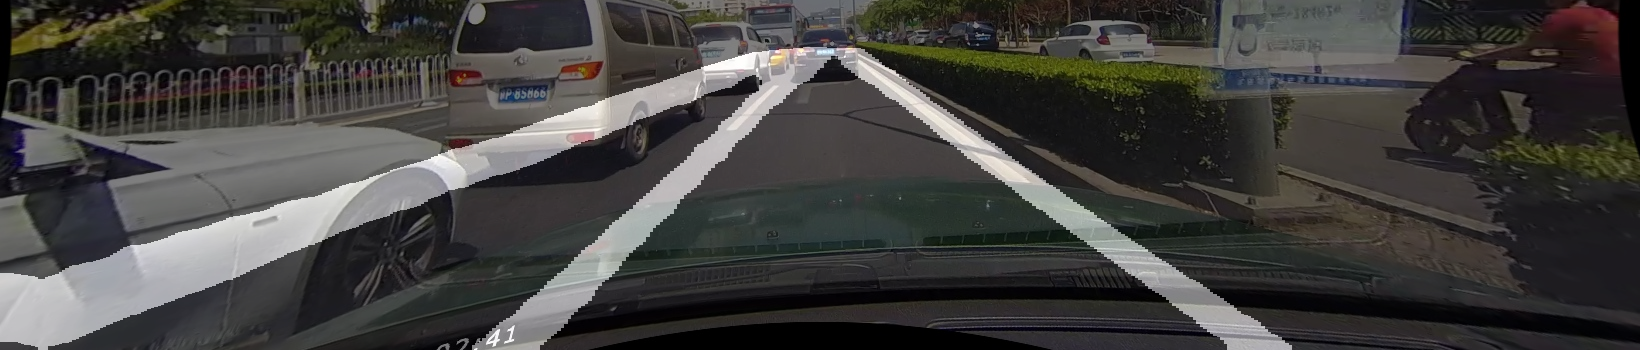
\includegraphics[width=1.2\linewidth, height=3cm]{images/SCNN_res_culane.png} 
                \caption{}
                \label{fig:subim1}
        \end{subfigure}
        \begin{subfigure}{0.4\textwidth}
                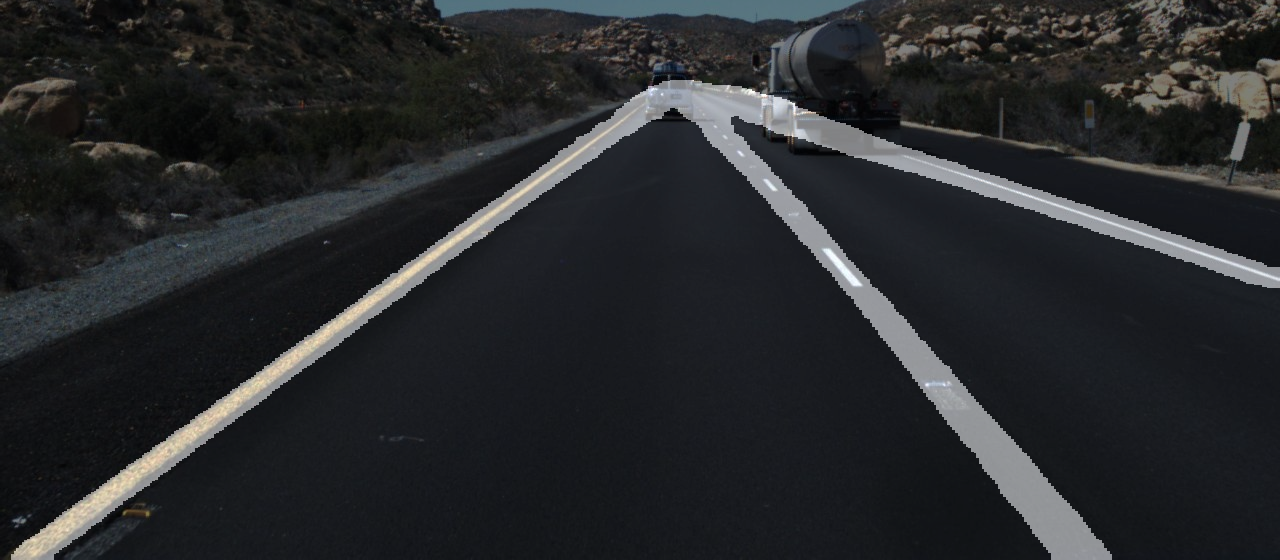
\includegraphics[width=1.2\linewidth, height=4cm]{images/SCNN_res_tusimple.png}
                \caption{}
                \label{fig:subim2}
        \end{subfigure}
        \newline
        \begin{subfigure}{0.4\textwidth}
                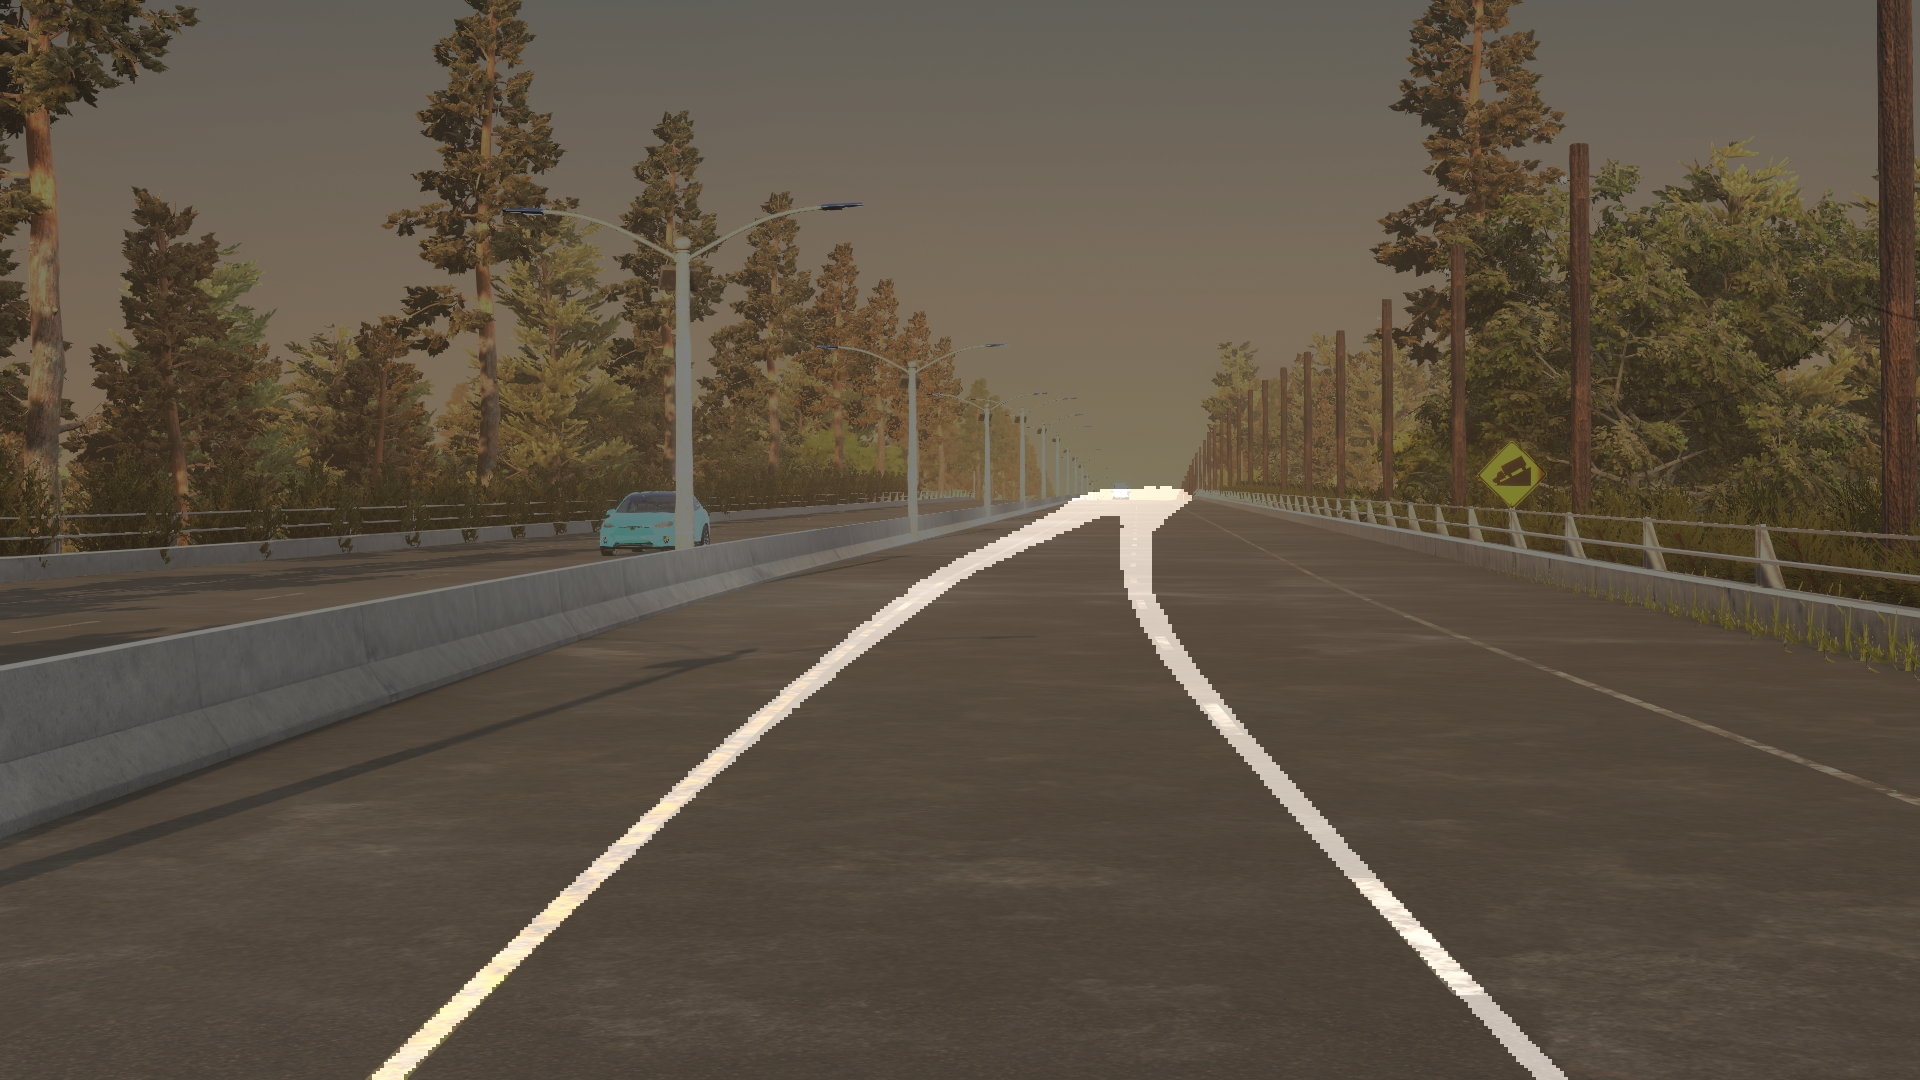
\includegraphics[width=1.2\linewidth, height=4cm]{images/Resa_r18_sim3d.png}
                \caption{}
                \label{fig:subim2}
        \end{subfigure}
        \label{fig:image2}
        \end{figure}
    
        From equation 4.1, cross-entropy loss aims at reducing the pixel-wise error. Therefore, cross-entropy only considers loss locally not globally. Thus the statistical distribution of labels can affect the overall loss. The cases where the occurrence of one class overpowers the other, this condition is called a class imbalance. Binary lane segmentation also suffers from the same problem as the number of pixels occupied by lane lines is far less than the number of pixels represented by the background. 
    
    Addressing this issue of class imbalance in binary lane segmentation, we conducted some experiments by replacing Cross Entropy loss with Dice loss and Focal loss. A detailed explanation of these losses is mentioned in section 4.1.2.
    
     \begin{table}[h!]
    \caption{Quantitative results for binary lane segmentation trained on sim3d \cite{guo2020gen} dataset using Cross Entropy Loss, Focal Loss and Dice Loss}
    \centering
    \begin{tabular}{|l|l|l|}
    \hline
        \textbf{Method} & \textbf{IoU} & \textbf{FPS} \\ \hline
        RESA(Res18+Cross Entropy) \cite{DBLP:journals/corr/abs-2008-13719} & 71.79 & $\approx$ 45 \\ \hline
        SCNN(Res18+Cross Entropy) \cite{pan2018SCNN} & 44.12 & $\approx$ \textbf{70}  \\ \hline
        RESA(Res50+Cross Entropy) \cite{DBLP:journals/corr/abs-2008-13719} & 74.11 & $\approx$ 40  \\ \hline

        RESA(Res18+Dice Loss) \cite{DBLP:journals/corr/abs-2008-13719}& 82.57 & $\approx$ 50 \\\hline
        RESA(Res50+Dice Loss) \cite{DBLP:journals/corr/abs-2008-13719}& \textbf{83.33} & $\approx$ 50 \\\hline
    \end{tabular}
\end{table}
    
      \begin{figure}[h]
       \caption{Qualitative results for binary lane segmentation trained on sim3d dataset\cite{guo2020gen}: (a) RESA(Res18+Cross Entropy Loss) \cite{DBLP:journals/corr/abs-2008-13719} (b) RESA(Res18+Dice Loss) \cite{DBLP:journals/corr/abs-2008-13719} (c)RESA(Res18+Focal Loss) \cite{DBLP:journals/corr/abs-2008-13719}}
        
        \begin{subfigure}{0.4\textwidth}
        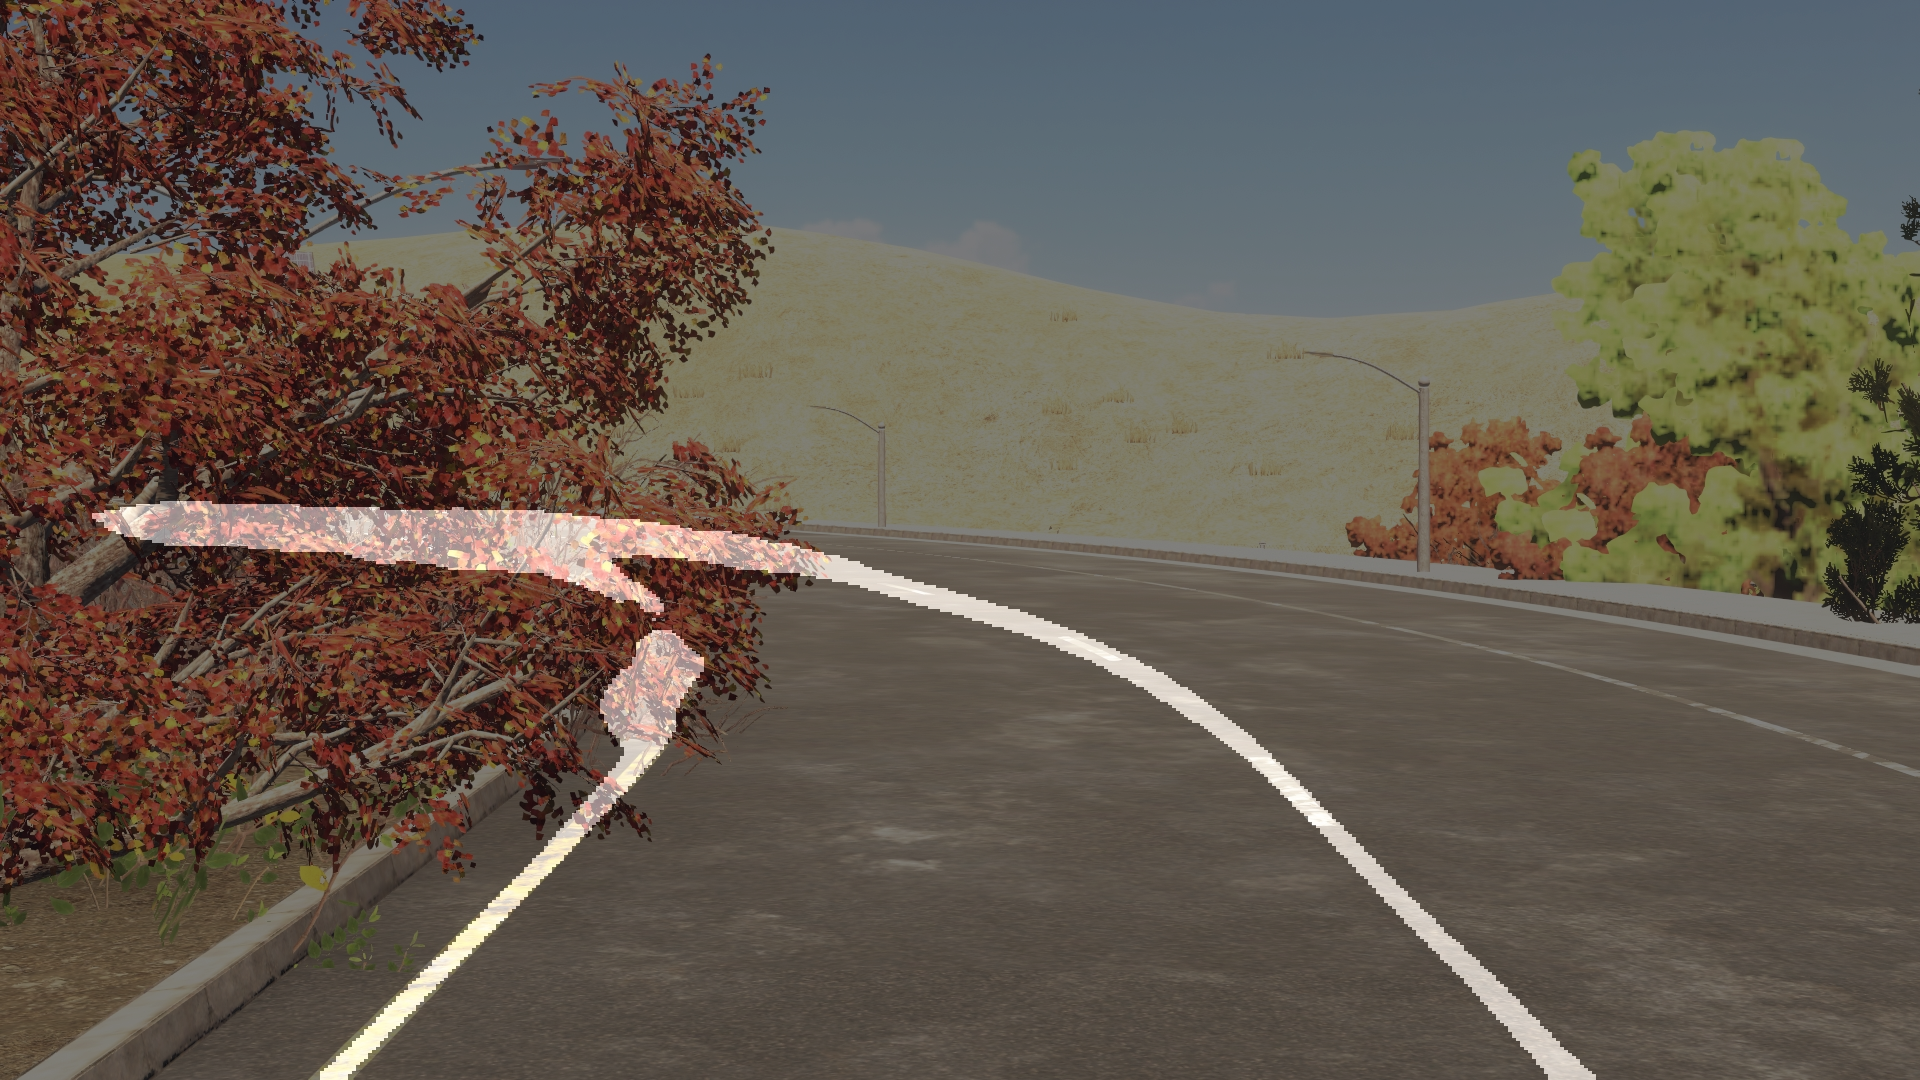
\includegraphics[width=1\linewidth, height=4cm]{images/binseg_ce_resa.png} 
        \caption{}
        \label{fig:subim1}
        \end{subfigure}
        \begin{subfigure}{0.4\textwidth}
        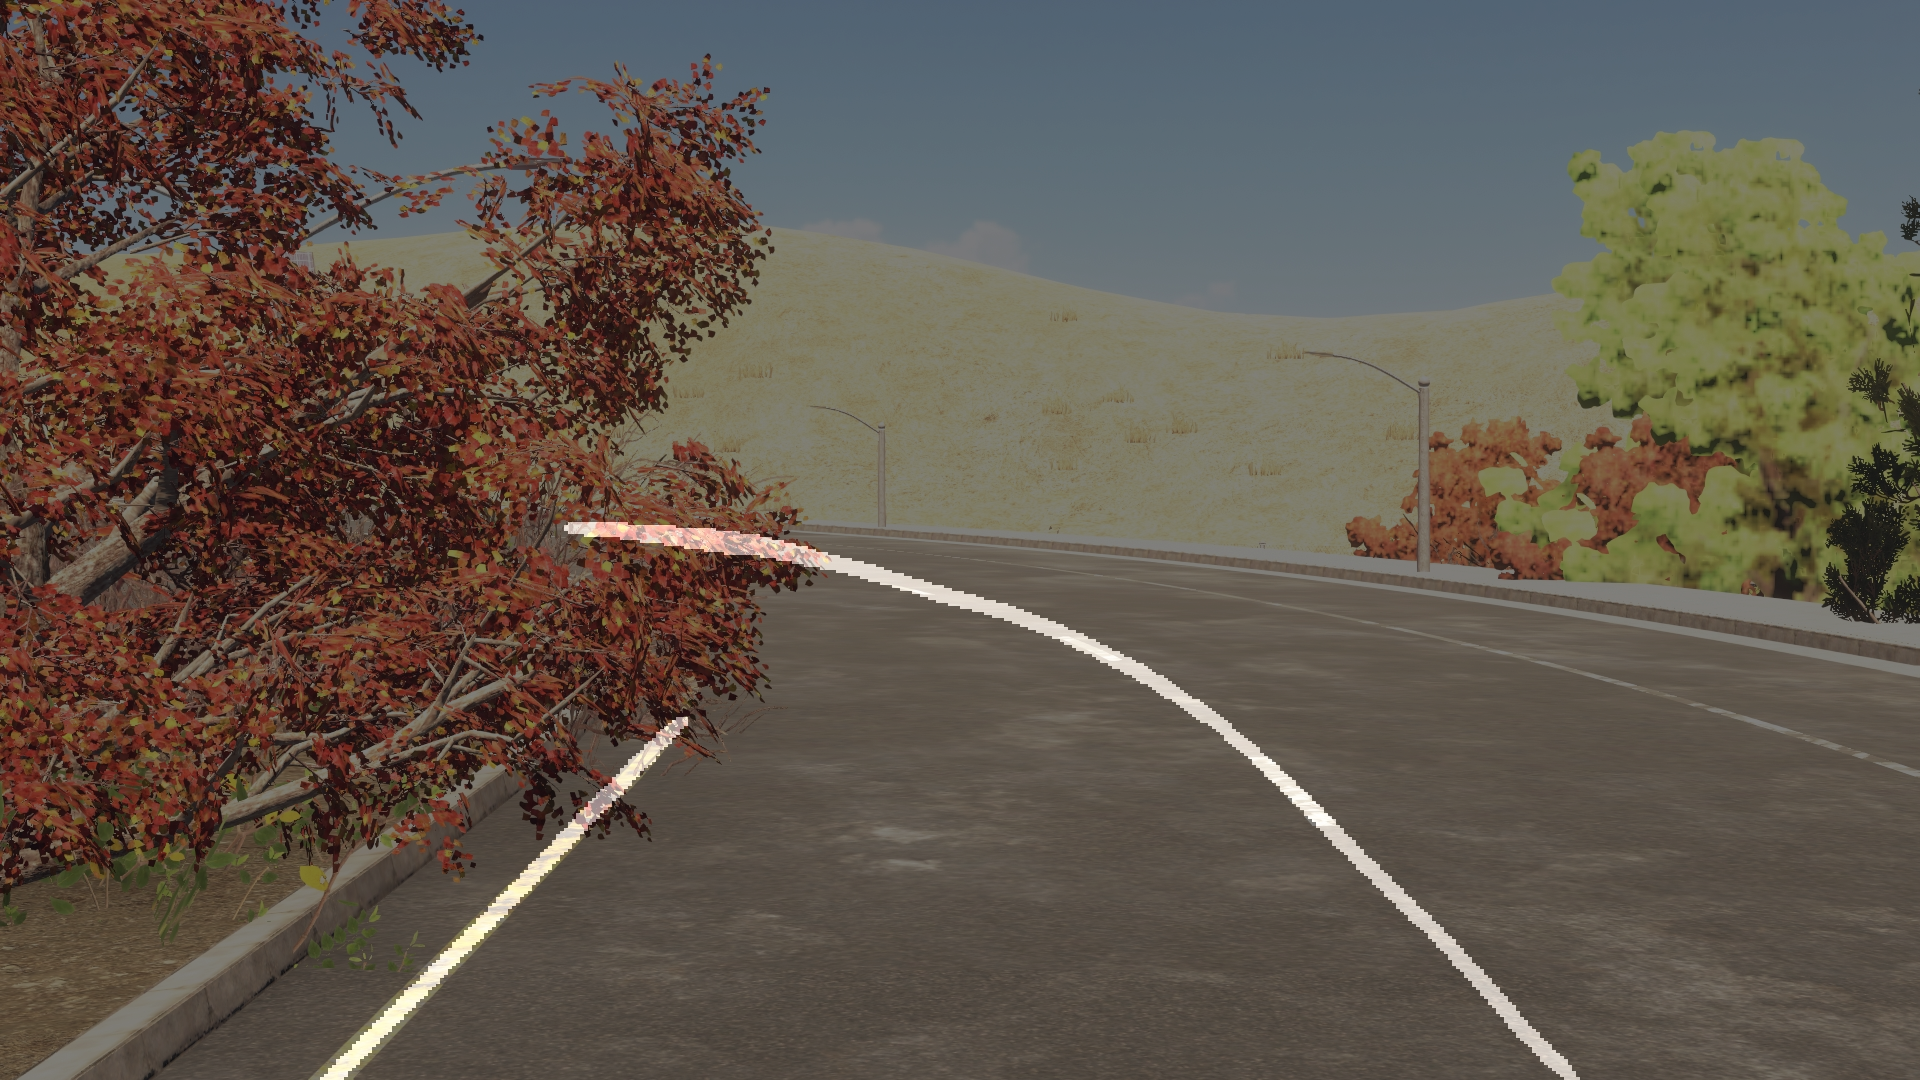
\includegraphics[width=1\linewidth,height=4cm]{images/binseg_dice_resa.png}
        \caption{}
        \label{fig:subim2}
        \end{subfigure}
        \begin{subfigure}{0.4\textwidth}
        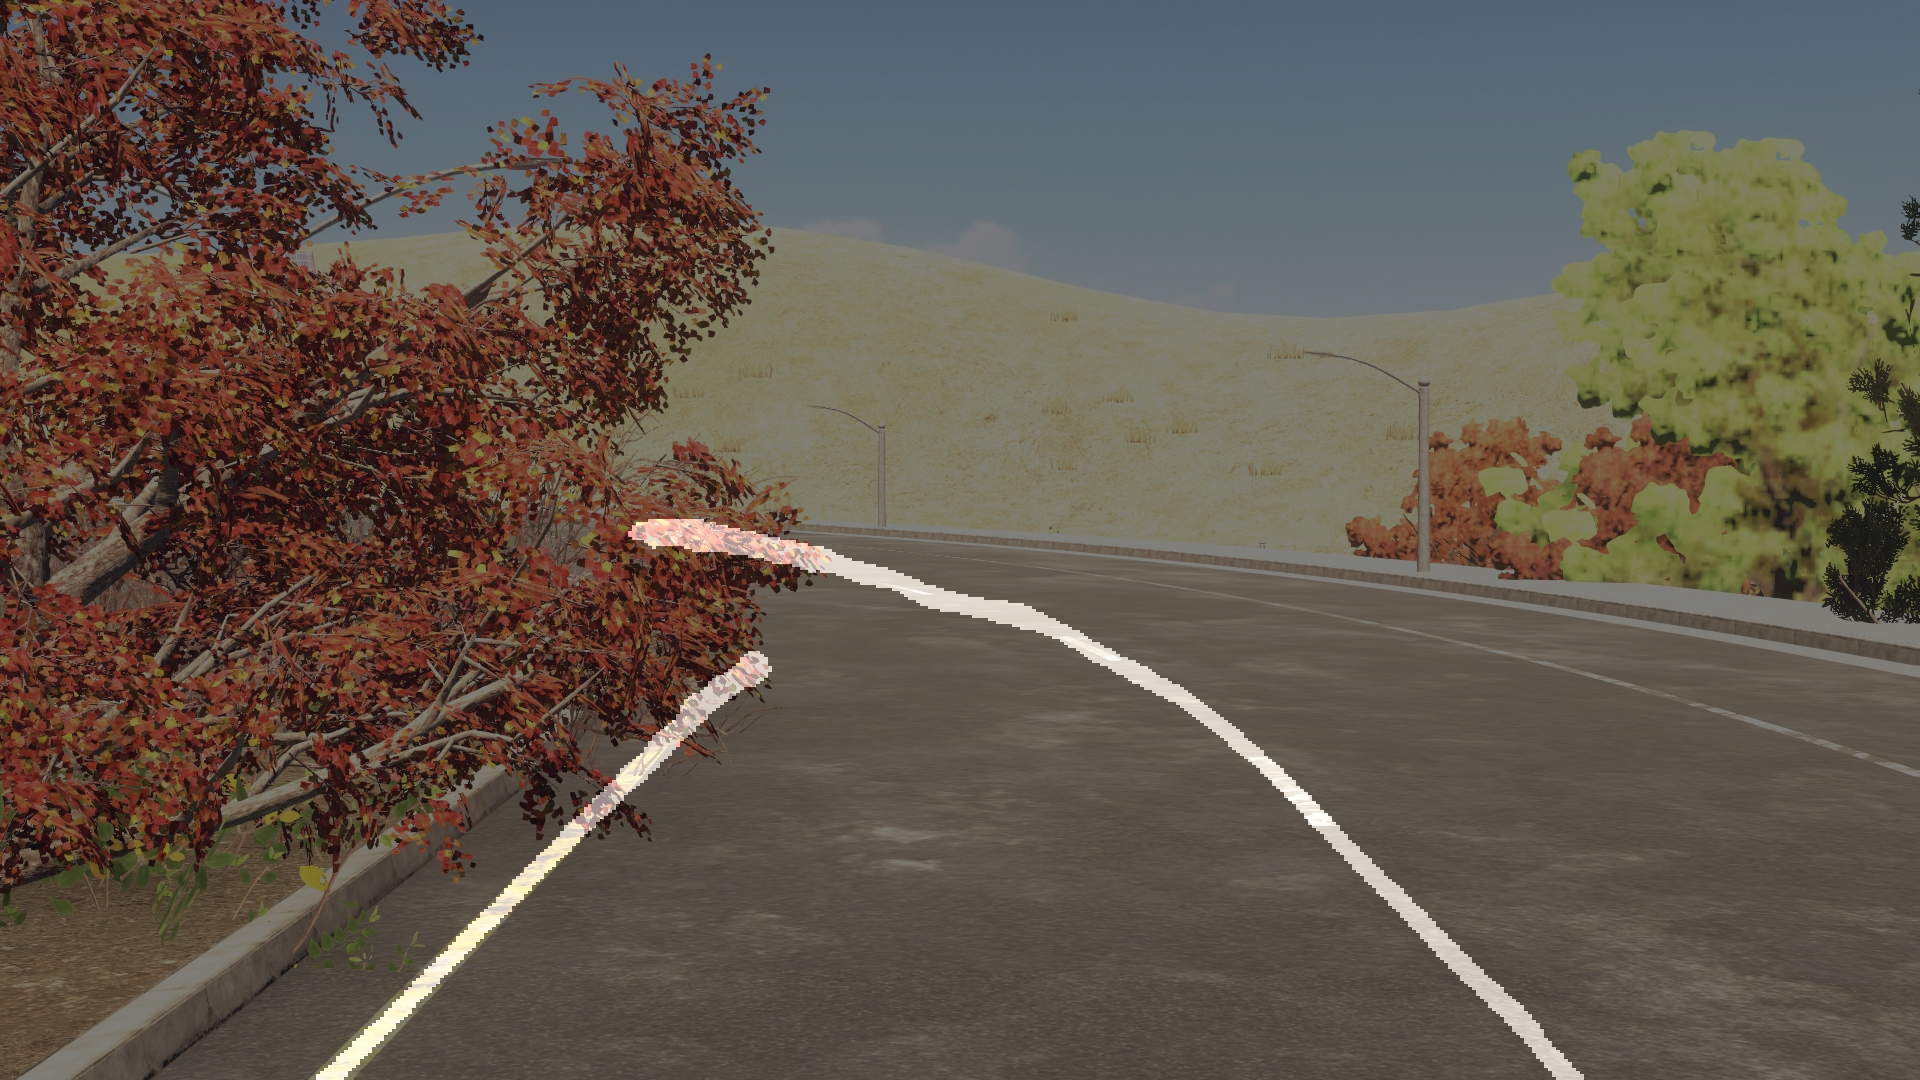
\includegraphics[width=1\linewidth, height=4cm]{images/binseg_focal_resa.png}
        \caption{}
        \label{fig:subim2}
        \end{subfigure}
        \label{fig:image2}
        \end{figure}
    
     \begin{figure}[h]
       \caption{IoU for ego-vehicle binary lane segmentation trained on sim3D dataset\cite{guo2020gen} with cross entropy, dice and focal loss.}
        \centering
        \begin{subfigure}{0.6\textwidth}
        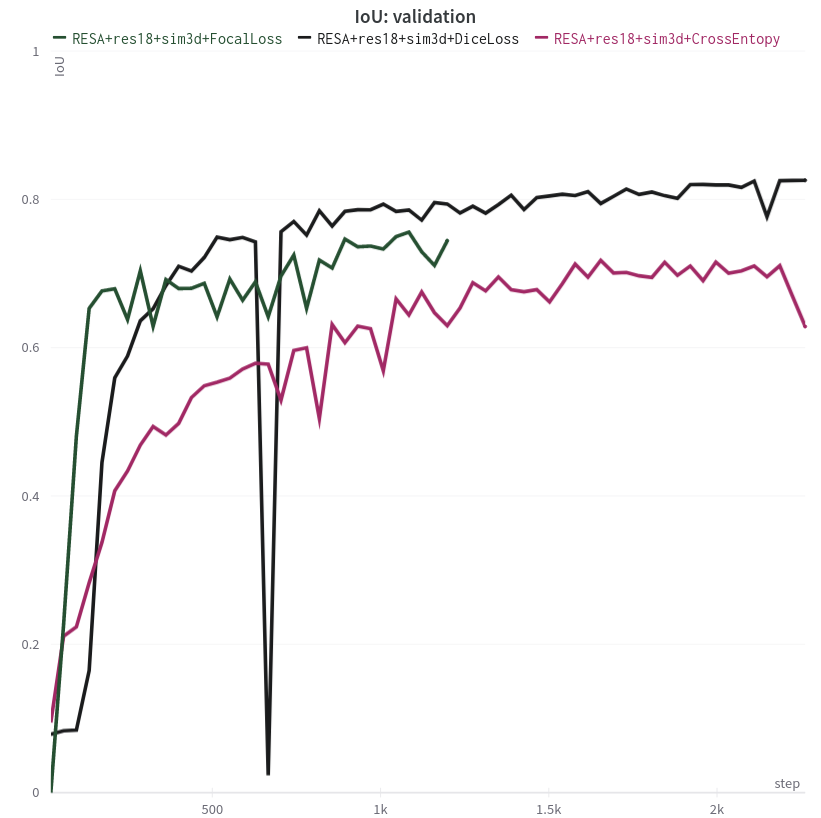
\includegraphics[width=1\linewidth, height=7cm]{images/change2.png} 
        \label{fig:subim1}
        \end{subfigure}
        \end{figure}
    
    From Table 5.3 and figure 5.3 we can conclude that using dice loss and focal loss the class imbalance problem is addressed, resulting in better IoU. Moreover, there is a significant improvement in the quality of binary lane segmentation.
    
        After countering the class imbalance problem we trained some models on sim3D dataset which predict binary lane segmentation for all the lanes present in the scene.
        
        \begin{figure}[h]
       \caption{IoU for binary lane segmentation trained on sim3D dataset with cross entropy, dice and focal loss.}
        \centering
        \begin{subfigure}{0.6\textwidth}
        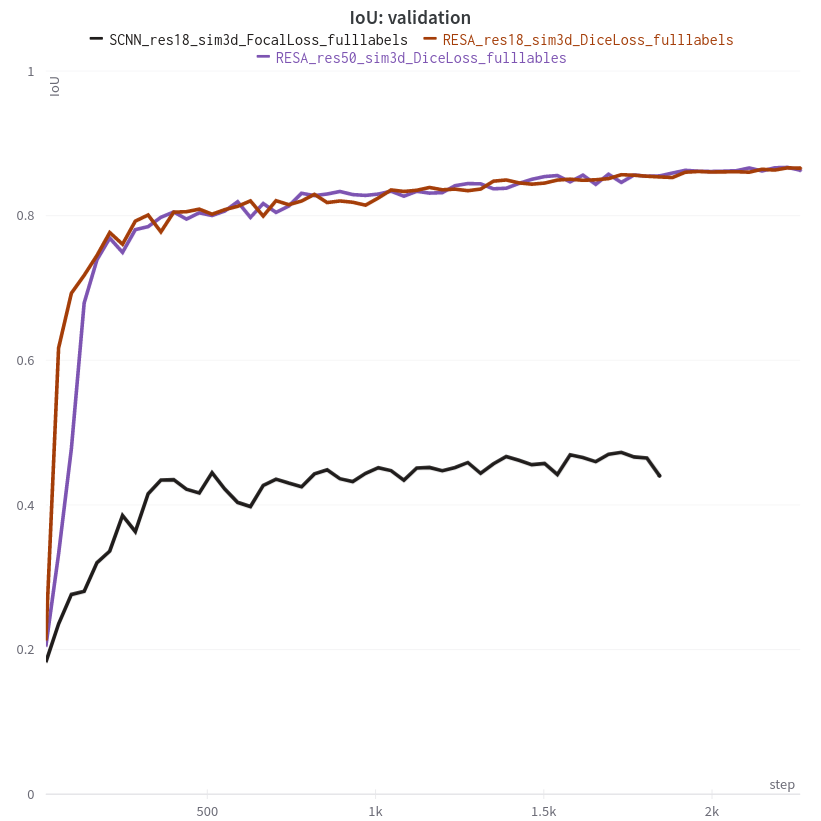
\includegraphics[width=1\linewidth, height=7cm]{images/change1.png} 
        \label{fig:subim1}
        \end{subfigure}
        \end{figure}
           
           \begin{table}[h]
    \caption{Quantitative results for binary lane segmentation on sim3D dataset \cite{guo2020gen} for all the lanes present in the scene for all the lanes present in the scene.}
    \centering
    \begin{tabular}{|l|l|l|}
    \hline
        \textbf{Method} & \textbf{IoU} & \textbf{FPS} \\ \hline
        SCNN(Res18+Focal Loss) \cite{pan2018SCNN}& 44.01 & $\approx$ \textbf{70} \\\hline
        RESA(Res18+Dice Loss) \cite{DBLP:journals/corr/abs-2008-13719}& 86.56 & $\approx$ 55 \\\hline
        RESA(Res50+Dice Loss) \cite{DBLP:journals/corr/abs-2008-13719}& \textbf{86.67} & $\approx$ 50 \\\hline
    \end{tabular}
\end{table}
From table 5.4, we can infer that RESA \cite{DBLP:journals/corr/abs-2008-13719} with ResNet50 as a backbone and using dice loss as an objective function we are able to obtain the best IoU of $86.67$ for the task of prediction binary lane segmentation masks on the sim3D dataset \cite{guo2020gen} and the qualitative results from figure 5.5 follow this claim. 
        \begin{figure}[h]
      \caption{Qualitative results for binary lane segmentation trained on sim3d dataset \cite{guo2020gen} for all the lanes present in the scene: (a) SCNN(Res18+Focal Loss) \cite{pan2018SCNN} (b) RESA(Res18+Dice Loss) \cite{DBLP:journals/corr/abs-2008-13719} (c)RESA(Res18+Focal Loss) \cite{DBLP:journals/corr/abs-2008-13719}}
        \centering
        \begin{subfigure}{0.4\textwidth}
        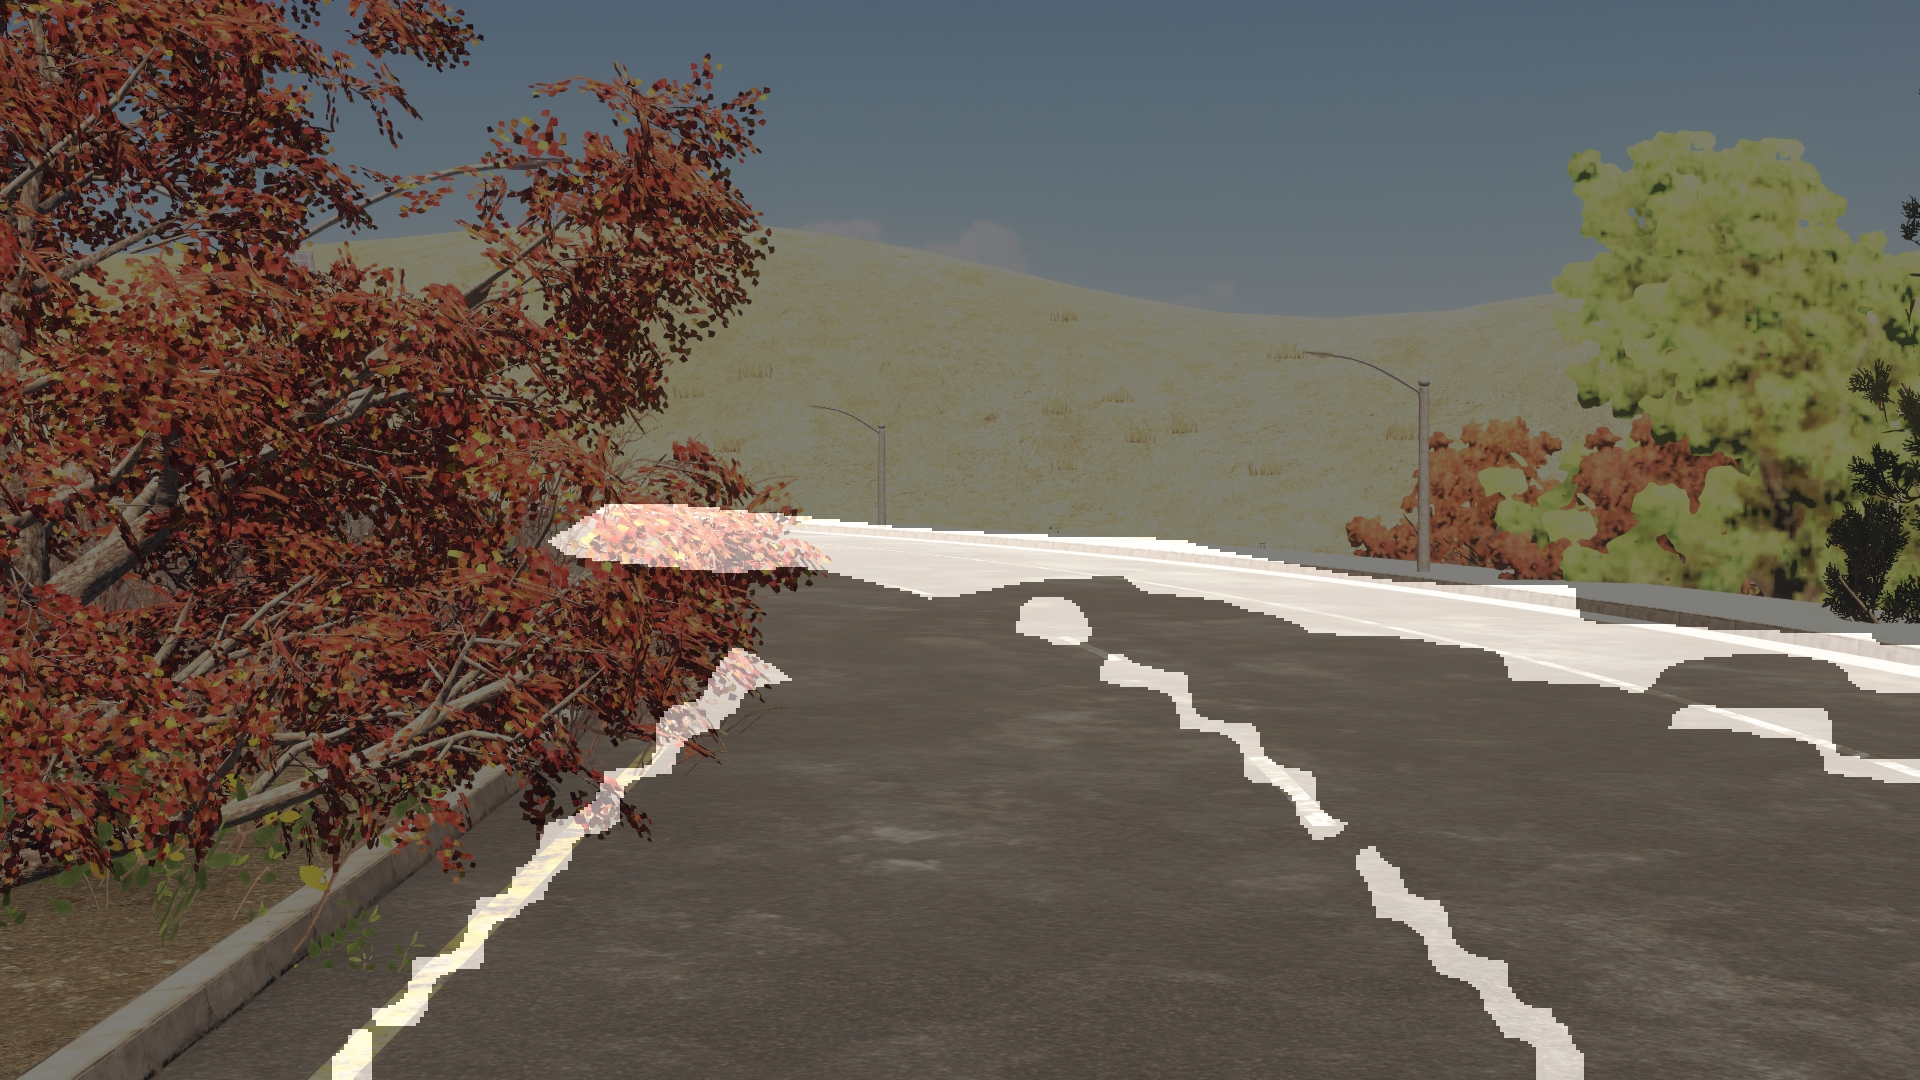
\includegraphics[width=1\linewidth, height=3.5cm]{images/full_res18_scnn_focal.png} 
        \caption{}
        \label{fig:subim1}
        \end{subfigure}
        \begin{subfigure}{0.4\textwidth}
        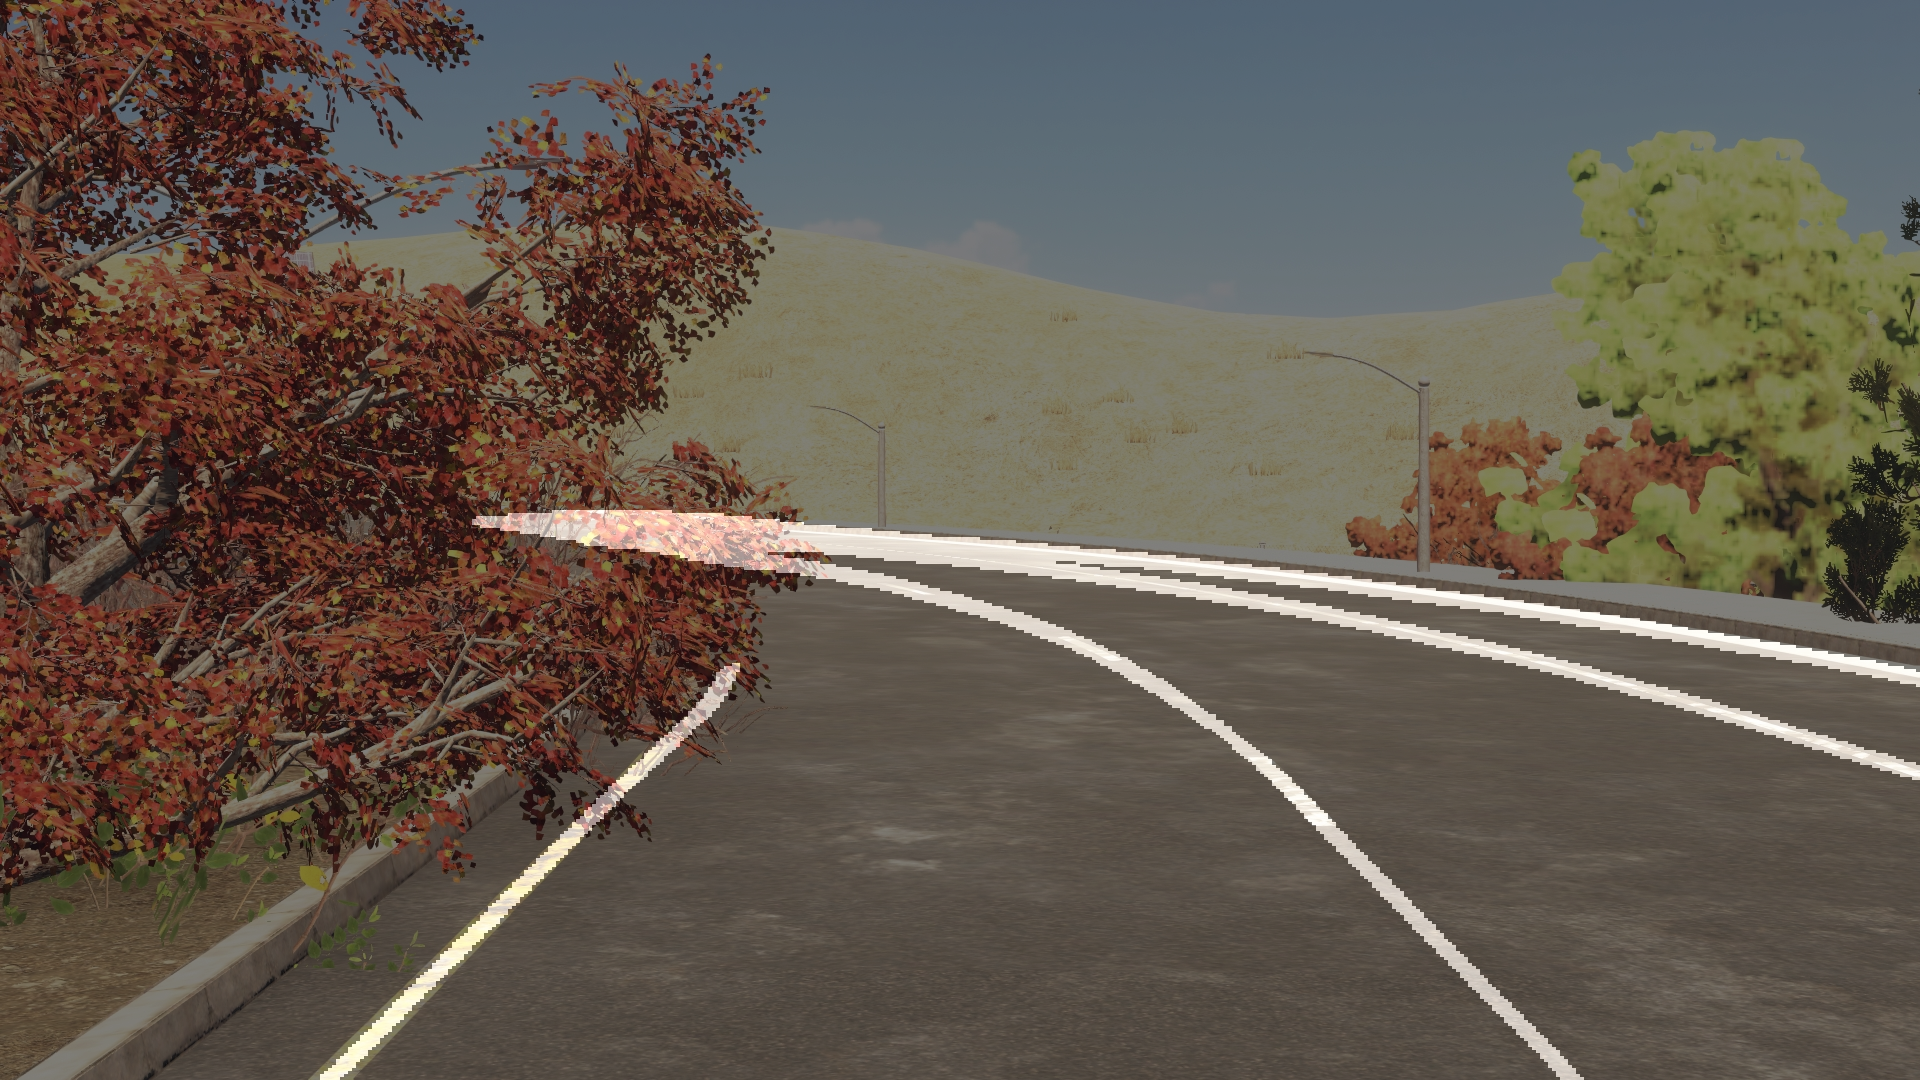
\includegraphics[width=1\linewidth,height=3.5cm]{images/Resa_r18_full_dice.png}
        \caption{}
        \label{fig:subim2}
        \end{subfigure}
        \begin{subfigure}{0.4\textwidth}
        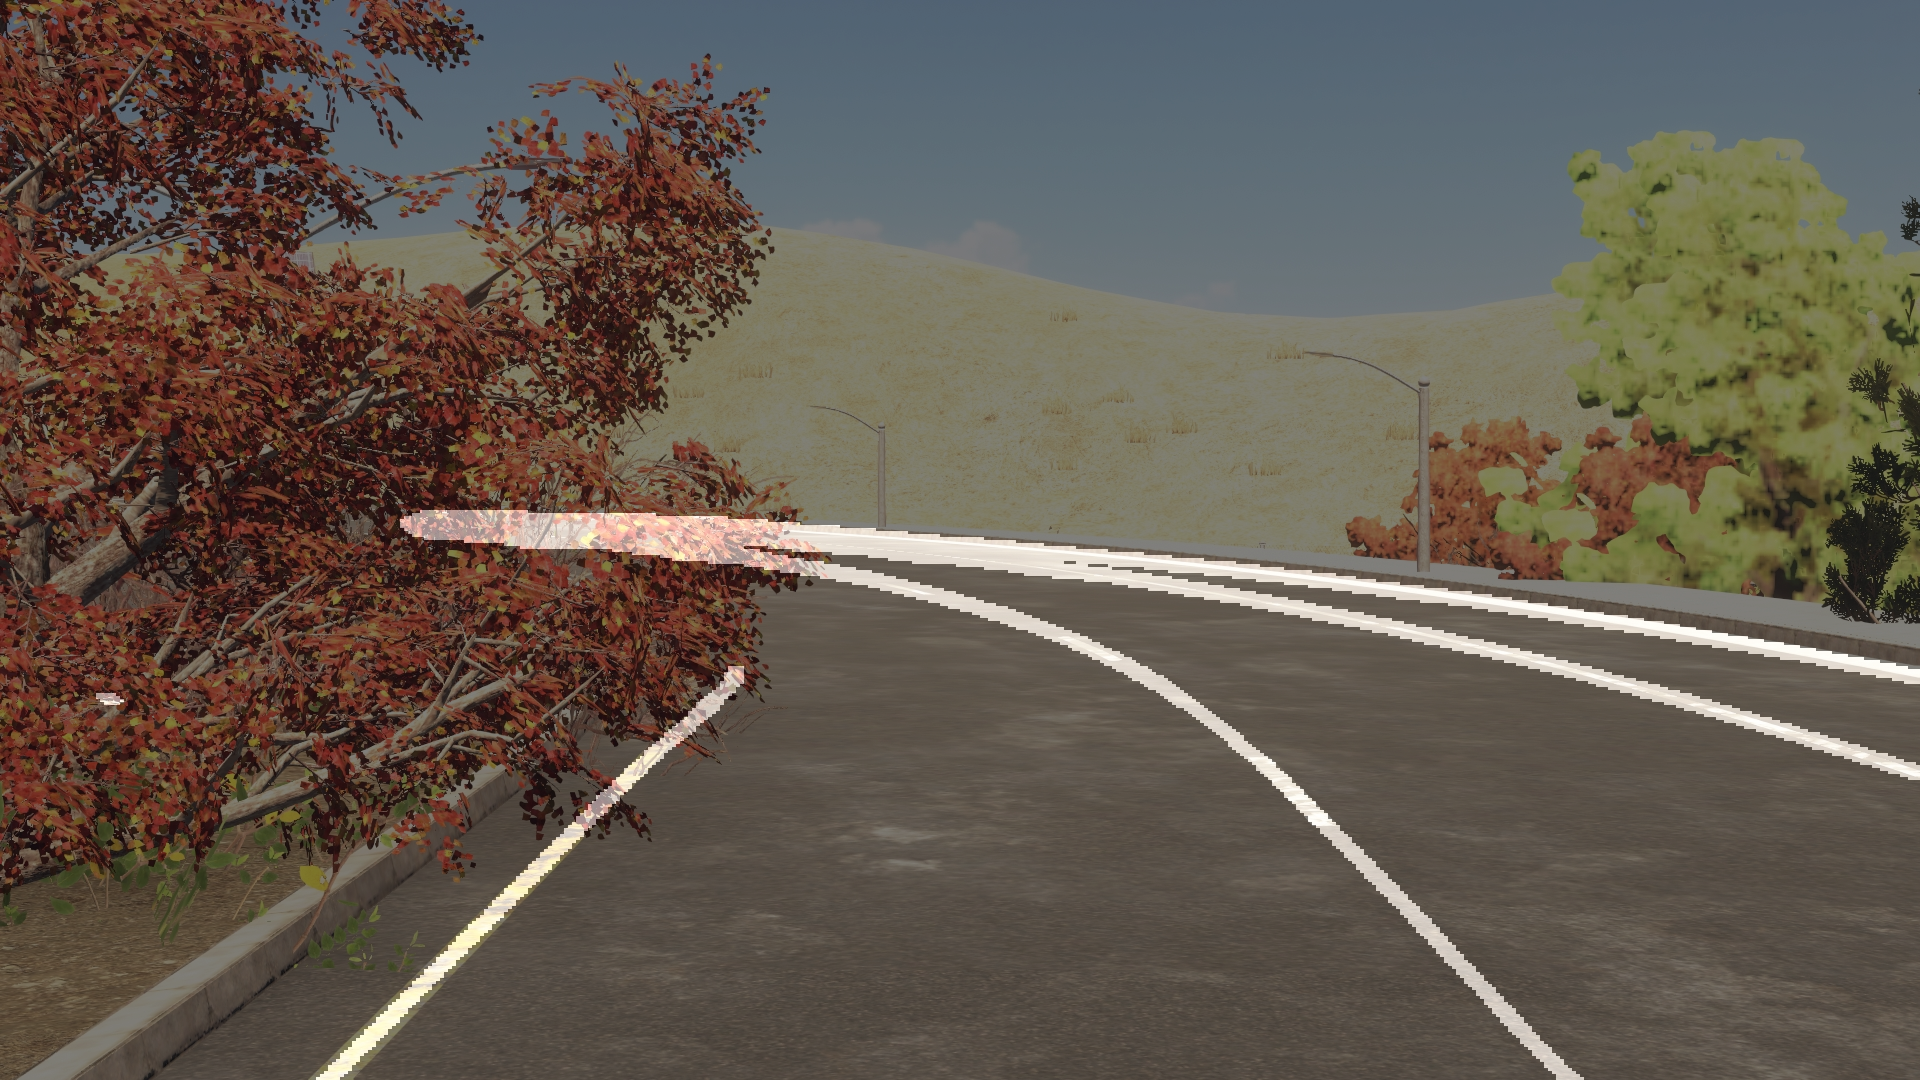
\includegraphics[width=1\linewidth, height=3.5cm]{images/Resa_r50_full_dice.png}
        \caption{}
        \label{fig:subim2}
        \end{subfigure}
        \label{fig:image2}
        \end{figure}
        
     From the above experiments, we have obtained an efficient binary lane segmentation algorithm that will facilitate our proposed dual-stage 3D lane detector. Binary lane segmentation is the first stage of the 3D lane detection pipeline any errors or uncertainties will be carried forward to the next stage of the 3D lane detection pipeline resulting in faulty detection. So it is necessary to have an efficient binary lane segmentation algorithm. 
    
        %---------------------------------------------------------------------%
    \section{3D Lane Detection}
    In this section, we will discuss in detail the effect of utilizing an efficient binary lane segmentation approach in a dual-stage manner of predicting 3D lane line points, and later on we will dive deeper into the challenges we are facing regarding the proposed dual-stage anchor-less semi-local 3D lane detector.  
    \subsection{Approach: 1}
    To check the efficacy and flexibility of the dual-stage manner of predicting 3D lanes using a complex binary lane segmentation model. We have conducted some experiments, where the dual-stage GenLaneNet \cite{guo2020gen} is trained using the best-performing binary lane segmentation algorithm obtained from section 5.2. 
    While training, the first stage of the 3D lane detection pipeline is fixed. Training and evaluation are carried out on a synthetic 3D lane dataset called sim3D \cite{guo2020gen}. The dataset is divided into three splits such that train and test sets have different distributions. Below we will discuss in detail quantitatively and qualitatively the results of training GenLaneNet \cite{guo2020gen} with a more complex binary lane segmentation algorithm on all the three splits of the sim3D dataset \cite{guo2020gen}.
 

    \begin{table}[htbp]
    \addtolength{\tabcolsep}{-1pt}
    \begin{center}
    \caption{Comparison between state of the art 3D lane detection approaches and the GenLaneNet \cite{guo2020gen} trained with complex binary lane segmentation architecture on balanced scenes from sim3D \cite{guo2020gen}, near range (0-40m) and far range (40-100m)}
    \begin{tabular}{|p{0.3\linewidth}|p{0.1\linewidth}|p{0.1\linewidth}|p{0.1\linewidth}|p{0.1\linewidth}|p{0.1\linewidth}|p{0.1\linewidth}|}
    \hline
        \textbf{Method} & \textbf{AP} & \textbf{F-Score} & \textbf{x error near(m)} & \textbf{x error far(m)} & \textbf{z error near(m)} & \textbf{z error far(m)} \\ \hline
        Gen-LaneNet\cite{guo2020gen} & 90.1 & 88.1 & 0.061 & 0.496 & 0.012 & 0.214 \\ \hline
        3D LaneNet \cite{DBLP:journals/corr/abs-1811-10203}& 89.3 & 86.4 & 0.068 & 0.477 & 0.015 & \textbf{0.202} \\ \hline
        CLGo \cite{DBLP:journals/corr/abs-2112-15351}& \textbf{94.2} &\textbf{ 91.9} & 0.061 & \textbf{0.361} & 0.029 & 0.250 \\ \hline
        3D-LaneNet(1/att) \cite{9506296} &  93.2 & 91.0 & 0.082 & 0.439 & \textbf{0.011} & 0.242 \\ \hline
        Gen-LaneNet(1/att) \cite{9506296}& 92.4 & 90.3 & 0.080 & 0.473 & \textbf{0.011} & 0.247 \\ \hline
        Gen-LaneNet(RESA+Res18) & 91.8 & 89.7 & \textbf{0.06} & 0.466 & 0.0114 & 0.24 \\ \hline
        Gen-LaneNet(RESA+Res50) & 92.2 & 90.2 &\textbf{ 0.06} & 0.461 & 0.0122 & 0.24 \\ \hline
    \end{tabular}
    \end{center}
    \end{table}
    
    Table 5.5 shows the comparison between state-of-the-art approaches for 3D lane detection and GenLaneNet \cite{guo2020gen} trained with more complex binary lane segmentation architecture on balanced scenes from sim3D dataset\cite{guo2020gen}. On the balanced scenes we are able to outperform GenLaneNet \cite{guo2020gen}, both AP and F-score are improved by \textbf{2.1}. In comparison with the other state-of-the-art approaches mentioned in table 5.5, we have achieved better results than 3DLaneNet \cite{DBLP:journals/corr/abs-1811-10203} and quite comparable results with respect to the other complex state-of-the-art approaches. 
        

        \begin{figure}[h]
      \caption{Qualitative results of the trained GenLaneNet\cite{guo2020gen} trained with complex binary lane segmentation architecture on balanced scenes from sim3D\cite{guo2020gen} dataset: (a) uphill (b) downhill scenario. The ground-truth lines are color coded in red and the predicted lanes in blue. }
        \centering
        \begin{subfigure}{1\textwidth}
        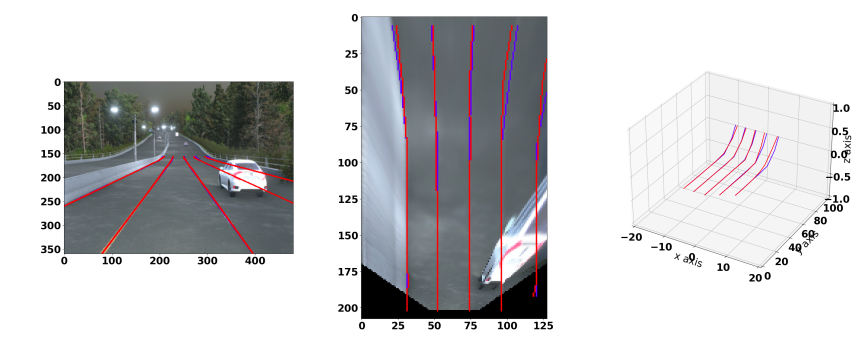
\includegraphics[width=1\linewidth, height=7cm]{images/uphill_standard.png} 
        \caption{  }
        \label{fig:subim1}
        \end{subfigure}
        \begin{subfigure}{1\textwidth}
        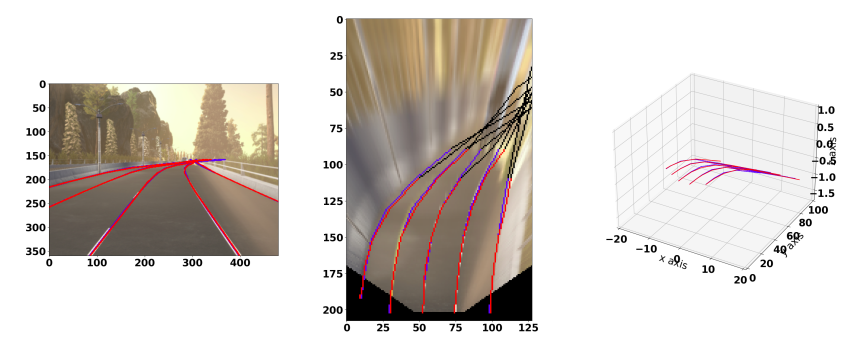
\includegraphics[width=1\linewidth,height=7cm]{images/downhill_standard.png}
        \caption{}
        \label{fig:subim2}
        \end{subfigure}
        \end{figure}


        \begin{table}[htbp]
    \centering
    \caption{Comparison between state of the art 3D lane detection approaches and the GenLaneNet \cite{Guo_2018_ECCV} trained with complex binary lane segmentation architecture on rarely observed scenes from sim3D \cite{guo2020gen}, near range (0-40m) and far range (40-100m)}
    \begin{tabular}{|p{0.3\linewidth}|p{0.1\linewidth}|p{0.1\linewidth}|p{0.1\linewidth}|p{0.1\linewidth}|p{0.1\linewidth}|p{0.1\linewidth}|}
    \hline
        \textbf{Method} & \textbf{AP} & \textbf{F-Score} & \textbf{x error near(m)} & \textbf{x error far(m)} & \textbf{z error near(m)} & \textbf{z error far(m)} \\ \hline
        Gen-LaneNet\cite{guo2020gen} & 79.0 & 78.0 & 0.139 & 0.903 & 0.030 & 0.539 \\ \hline
        3D LaneNet\cite{DBLP:journals/corr/abs-1811-10203} & 74.6 & 72.0 & 0.166 & 0.855 & 0.039 &\textbf{ 0.521} \\ \hline
        CLGo\cite{DBLP:journals/corr/abs-2112-15351} &\textbf{ 88.3} &\textbf{ 86.1} & 0.147 & \textbf{0.735} & 0.071 & 0.609 \\ \hline
        3D-LaneNet(1/att)\cite{9506296} & 85.8 & 84.1 & 0.289 & 0.925 &\textbf{ 0.025} & 0.625 \\ \hline
        Gen-LaneNet(1/att)\cite{9506296} & 83.2 & 81.7 & 0.283 & 0.915 & 0.028 & 0.653 \\ \hline
        Gen-LaneNet(RESA+Res18) &  84.9 & 83.2 &\textbf{ 0.135} & 0.886 & 0.0308 & 0.607 \\ \hline
        Gen-LaneNet(RESA+Res50) & 83.7 & 82.3 & 0.14 & 0.919 & 0.0283 & 0.604 \\ \hline
    \end{tabular}
\end{table}
    
     From table 5.6 we can infer that on the rarely observed scenes from sim3D dataset \cite{guo2020gen}, we are able to outperform GenLaneNet \cite{guo2020gen}, both AP and F-score are improved by \textbf{5.4} and \textbf{4.3} respectively. In comparison with the other state-of-the-art approaches mentioned in table 5.6, we have achieved better metrics than 3DLaneNet \cite{DBLP:journals/corr/abs-1811-10203}, Gen-LaneNet(1/att) \cite{9506296} and quite comparable results with respect to the other complex state of the approaches. 
    
    \begin{figure}[h]
      \caption{Qualitative results of the GenLaneNet\cite{guo2020gen} trained with complex binary lane segmentation architecture on rarely observed scenes from sim3D\cite{guo2020gen} dataset: (a) uphill (b) downhill scenario. The ground-truth lines are color-coded in red and the predicted lanes in blue.}
        \centering
        \begin{subfigure}{1\textwidth}
        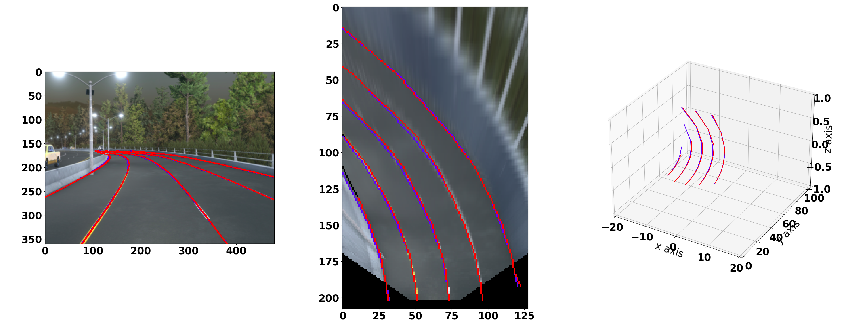
\includegraphics[width=1\linewidth, height=7cm]{images/uphill_rare.png} 
        \caption{}
        \label{fig:subim1}
        \end{subfigure}
        \begin{subfigure}{1\textwidth}
        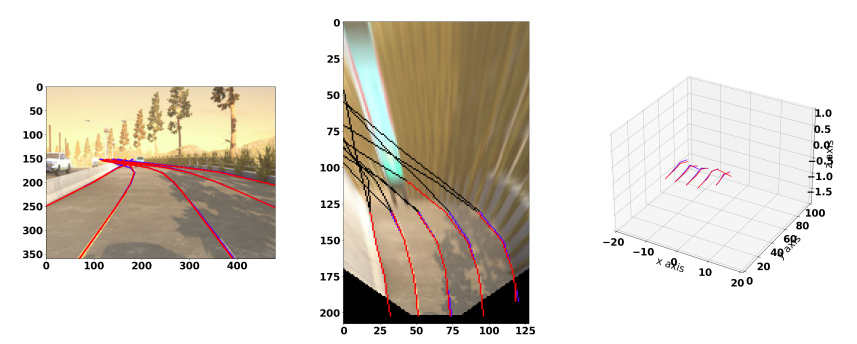
\includegraphics[width=1\linewidth,height=7cm]{images/downhill_rare.png}
        \caption{}
        \label{fig:subim2}
        \end{subfigure}
        \end{figure}
        
        \begin{table}[h]
    \centering
    \caption{Comparison between state of the art 3D lane detection approaches and the GenLaneNet \cite{guo2020gen} trained with complex binary lane segmentation architecture on scenes with visual variations from sim3D \cite{guo2020gen}, near range (0-40m) and far range (40-100m)}
    \begin{tabular}{|p{0.3\linewidth}|p{0.1\linewidth}|p{0.1\linewidth}|p{0.1\linewidth}|p{0.1\linewidth}|p{0.1\linewidth}|p{0.1\linewidth}|}
    \hline
        \textbf{Method} & \textbf{AP} & \textbf{F-Score} & \textbf{x error near(m)} & \textbf{x error far(m)} & \textbf{z error near(m)} & \textbf{z error far(m)} \\ \hline
        Gen-LaneNet\cite{guo2020gen} & 87.2 & 85.3 & 0.074 & 0.538 & 0.015 & 0.232 \\ \hline
        3D LaneNet\cite{DBLP:journals/corr/abs-1811-10203} & 74.9 & 72.5 & 0.115 & 0.601 & 0.032 & \textbf{0.230} \\ \hline
        CLGo \cite{DBLP:journals/corr/abs-2112-15351}& 89.2 & 87.3 & 0.084 & \textbf{0.464} & 0.045 & 0.312 \\ \hline
        3D-LaneNet(1/att) \cite{9506296} & 87.4 & 85.4 & 0.118 & 0.559 & 0.018 & 0.290 \\ \hline
        Gen-LaneNet(1/att) \cite{9506296}& 88.5 & 86.8 & 0.104 & 0.544 & 0.016 & 0.294 \\ \hline
        Gen-LaneNet(RESA+Res18) & \textbf{ 91.1} &\textbf{ 89.2} & 0.734 & 0.496 & \textbf{0.0134} & 0.259 \\ \hline
        Gen-LaneNet(RESA+Res50) & 90.7 & 88.8 & \textbf{0.0653} & 0.477 & 0.014 & 0.258 \\ \hline
    \end{tabular}
\end{table}

 From table 5.7 we can infer that on the scenes with visual variants from sim3D dataset \cite{guo2020gen}, we are able to outperform GenLaneNet \cite{guo2020gen}, both AP and F-score are improved by \textbf{3.9} respectively. In comparison with the other state-of-the-art approaches mentioned in table 5.6, Gen-LaneNet(RESA+Res18) has outperformed all other approaches.
 
 From the above experimentation, we have shown that using a complex binary lane segmentation architecture can enhance the performance of the dual-stage 3D lane detection. Using a similar idea we have trained our proposed anchor-less semi-local dual stage 3D lane detector, thus making our solution more robust and flexible in choosing a better architecture for binary lane segmentation. The main motive of the above-mentioned experimentation is to make sure that the first stage of the 3D lane detection algorithm is more robust toward any inference errors which will propagate in the later stages of the pipeline. 

\begin{figure}[h]
      \caption{Qualitative results of the  GenLaneNet\cite{guo2020gen} trained with complex binary lane segmentation architecture on visually varied scenes from sim3D\cite{guo2020gen} dataset: (a) uphill (b) downhill scenario. The ground-truth lines are color-coded in red and the predicted lanes in blue.}
        \centering
        \begin{subfigure}{1\textwidth}
        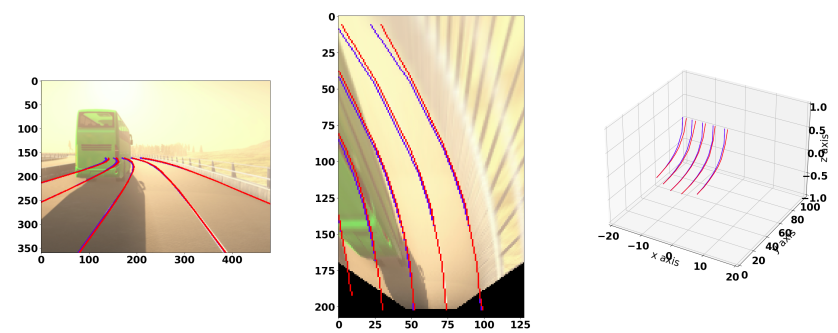
\includegraphics[width=1\linewidth, height=7cm]{images/uphill_illus.png} 
        \caption{}
        \label{fig:subim1}
        \end{subfigure}
        \begin{subfigure}{1\textwidth}
        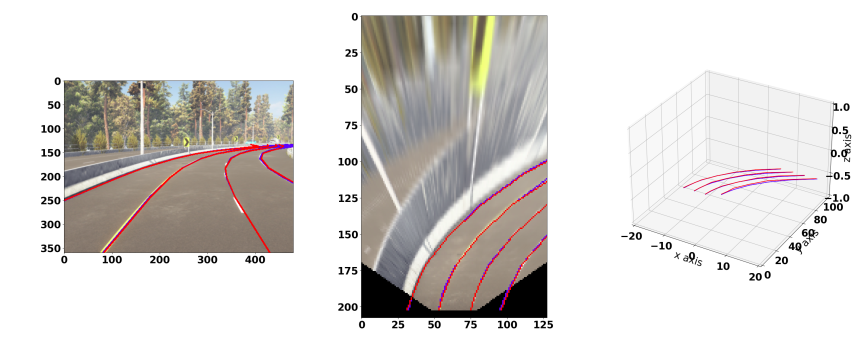
\includegraphics[width=1\linewidth,height=7cm]{images/downhill_illus.png}
        \caption{}
        \label{fig:subim2}
        \end{subfigure}
        \end{figure}
        
        
\subsection{Approach: 2}
In this section, we will discuss the challenges that we are facing currently in our proposed dual-stage anchor-less semi-local 3D lane detector. We have utilized the best-performing model from table 5.3 for the first stage which is responsible for predicting binary lane segmentation masks from an input image. Doing this has ensured that using the first stage of the proposed approach is not a bottleneck towards obtaining robust 3D lane line points. While training the proposed pipeline on the sim3D dataset for obtaining 3D lane line points, we observed that there was a discrepancy in the geometric representation of the lanes. Before delving deeper into that we will discuss the experiments that we have conducted for training the regression and embedding pathway. For a detailed explanation of the functionality of both the pathways and which loss functions are used to train them you can refer to section 4.2.5. 

Initially, during training we were using overall loss from the network as: 
\begin{equation}
    Overall loss = L_{regression} + L_{embedding} 
\end{equation}
After some experimental runs, we noticed that the embedding pathway was not learning efficiently as the magnitude of the loss from the regression pathway is large in comparison to the loss from the regression pathway. As the loss from both branches was summed to obtain the overall loss, the training signals were not meaningful enough to train the embedding pathway. Therefore we changed our schema to calculate the overall loss:

\begin{equation}
    Overall loss = w_{regression} * L_{regression} + w_{embedding} * L_{embedding} 
\end{equation}
 After switching to a weighted sum of losses from both the branches to calculate overall loss we performed some training runs and found that the same issue prevails. Figure 5.9 shows the activation maps of the convolutional layers from regression and embedding pathways when both branches are trained simultaneously using a weighted overall loss as an objective function. It can be seen that both the layers are not learning any meaningful information from the input binary lane segmentation mask.  
 
 \begin{figure}[h]
      \caption{Activation maps of convolutional layers (a) embedding pathway (b) regression pathway, while training them simultaneously}
        \centering
        \begin{subfigure}{0.8\textwidth}
        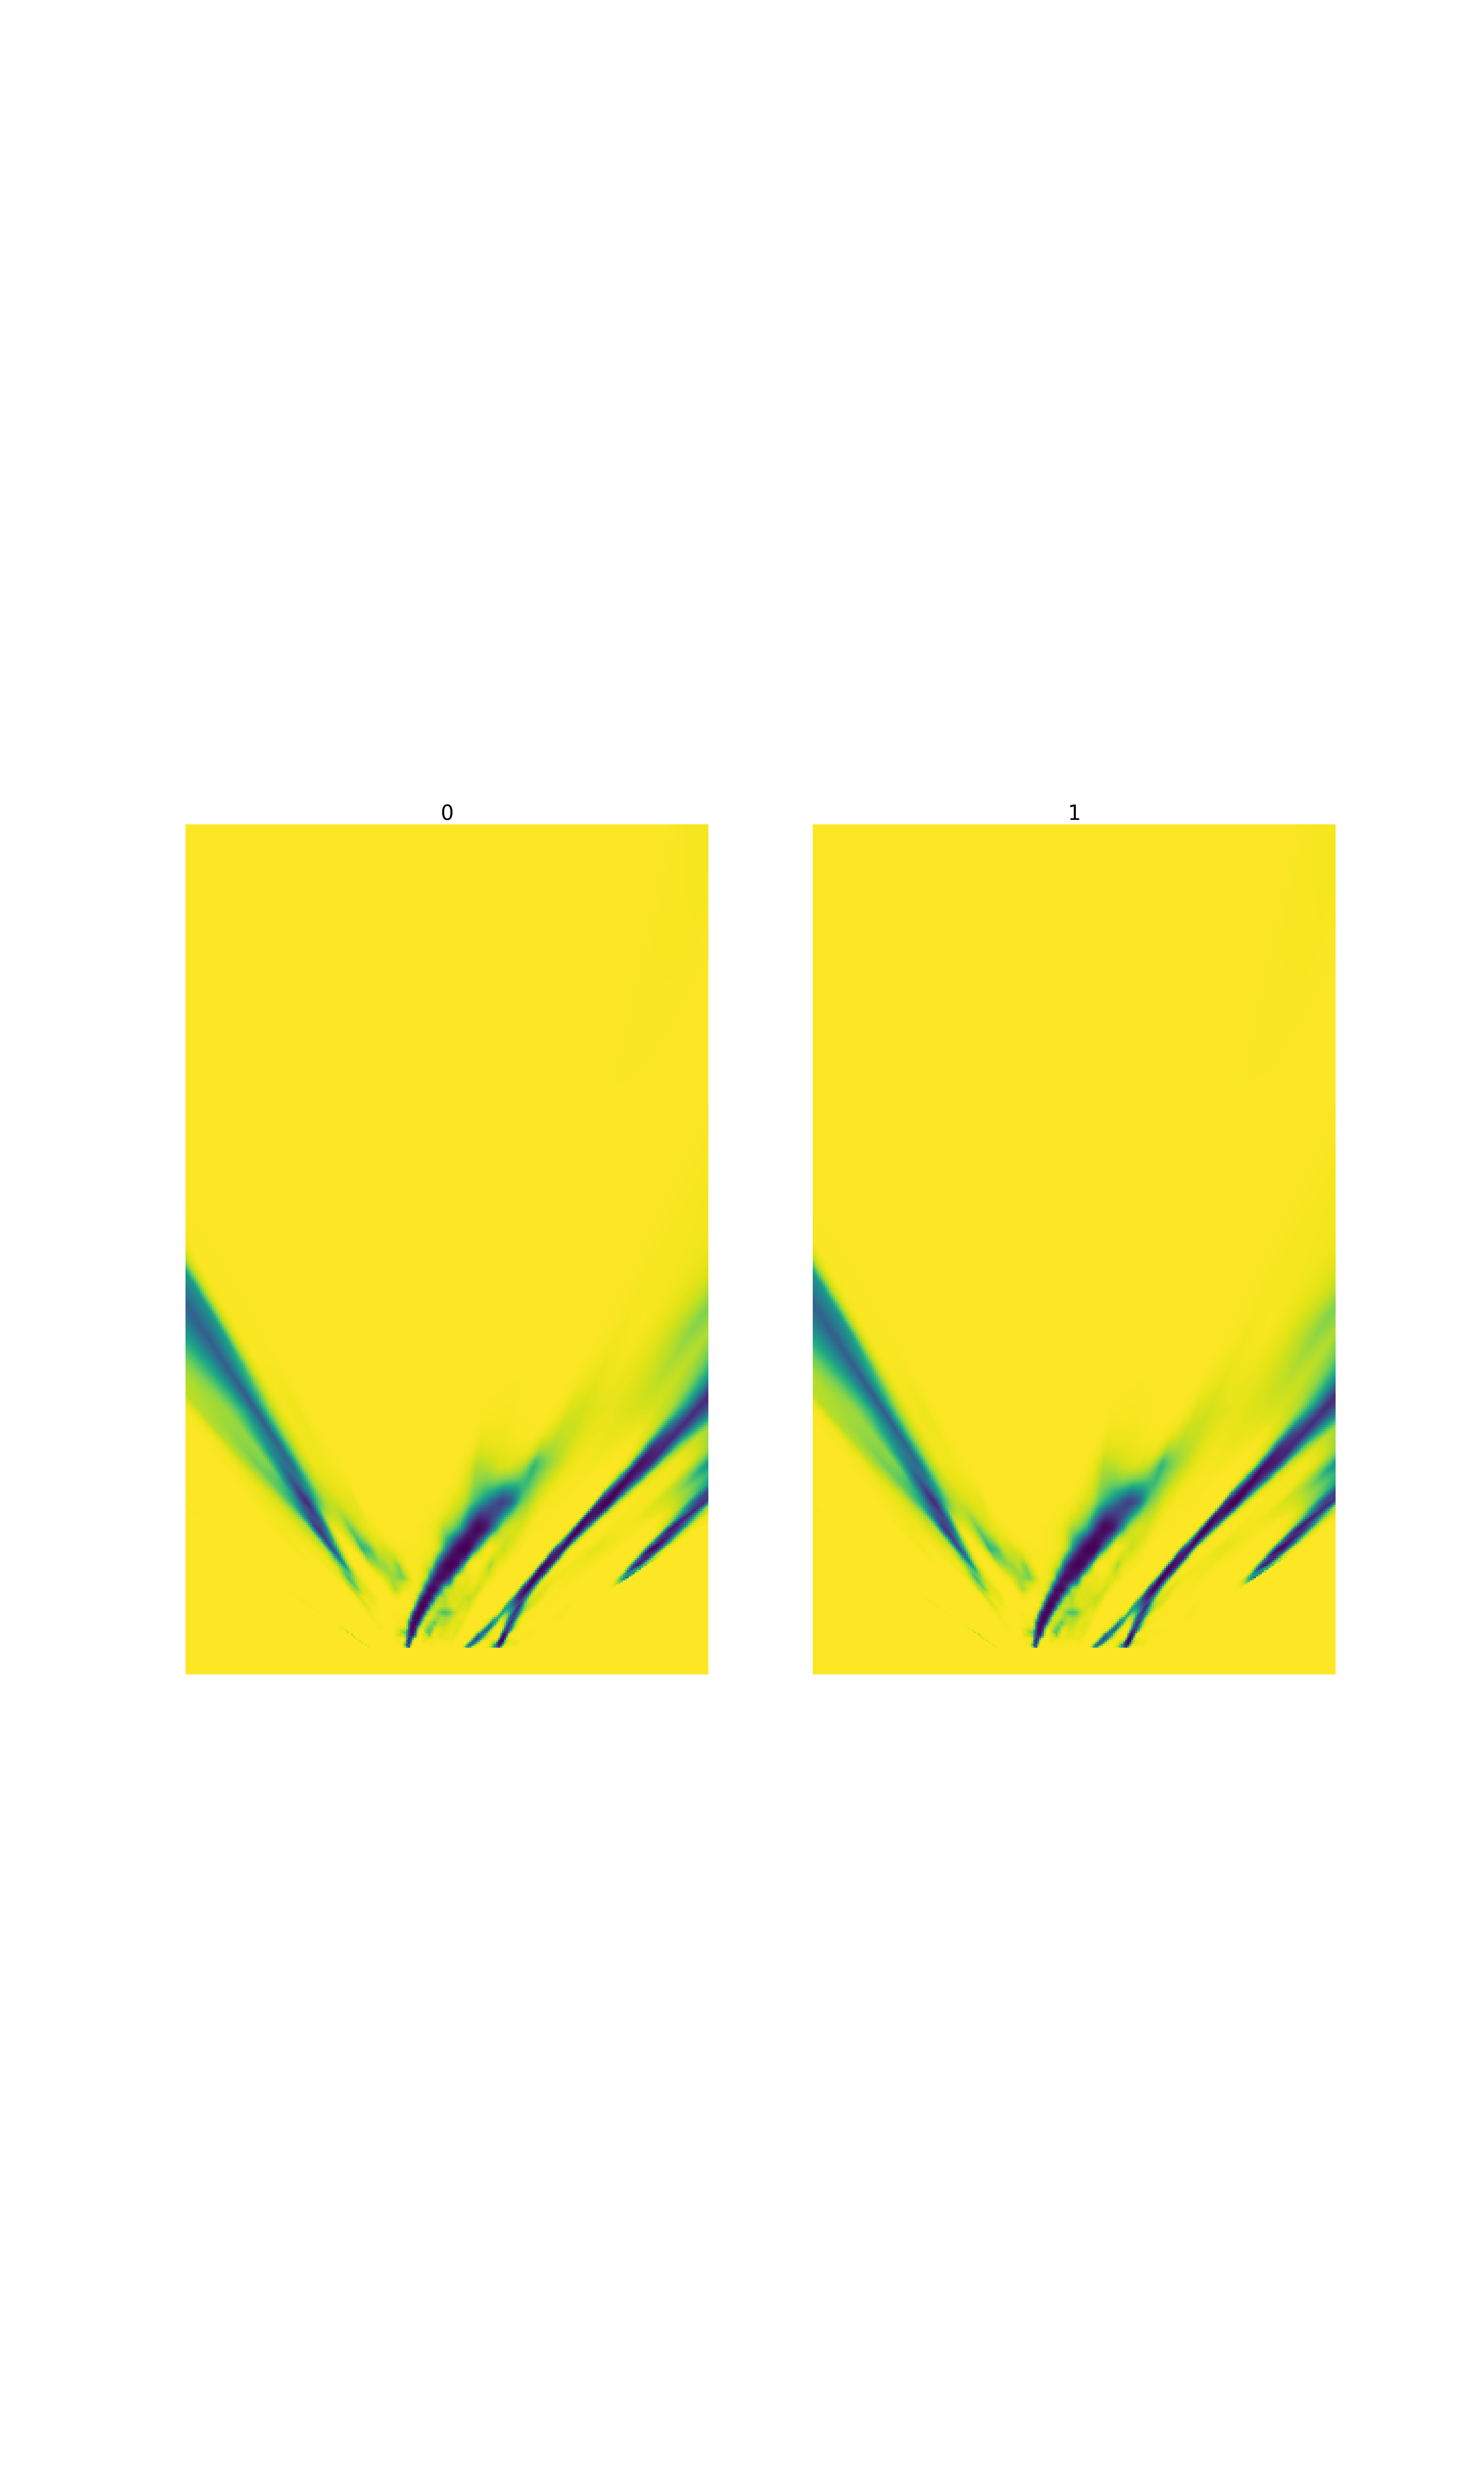
\includegraphics[width=1\linewidth, height=10cm]{images/activation_embededing_nofix.png} 
        \caption{}
        \label{fig:subim1}
        \end{subfigure}
        \begin{subfigure}{0.8\textwidth}
        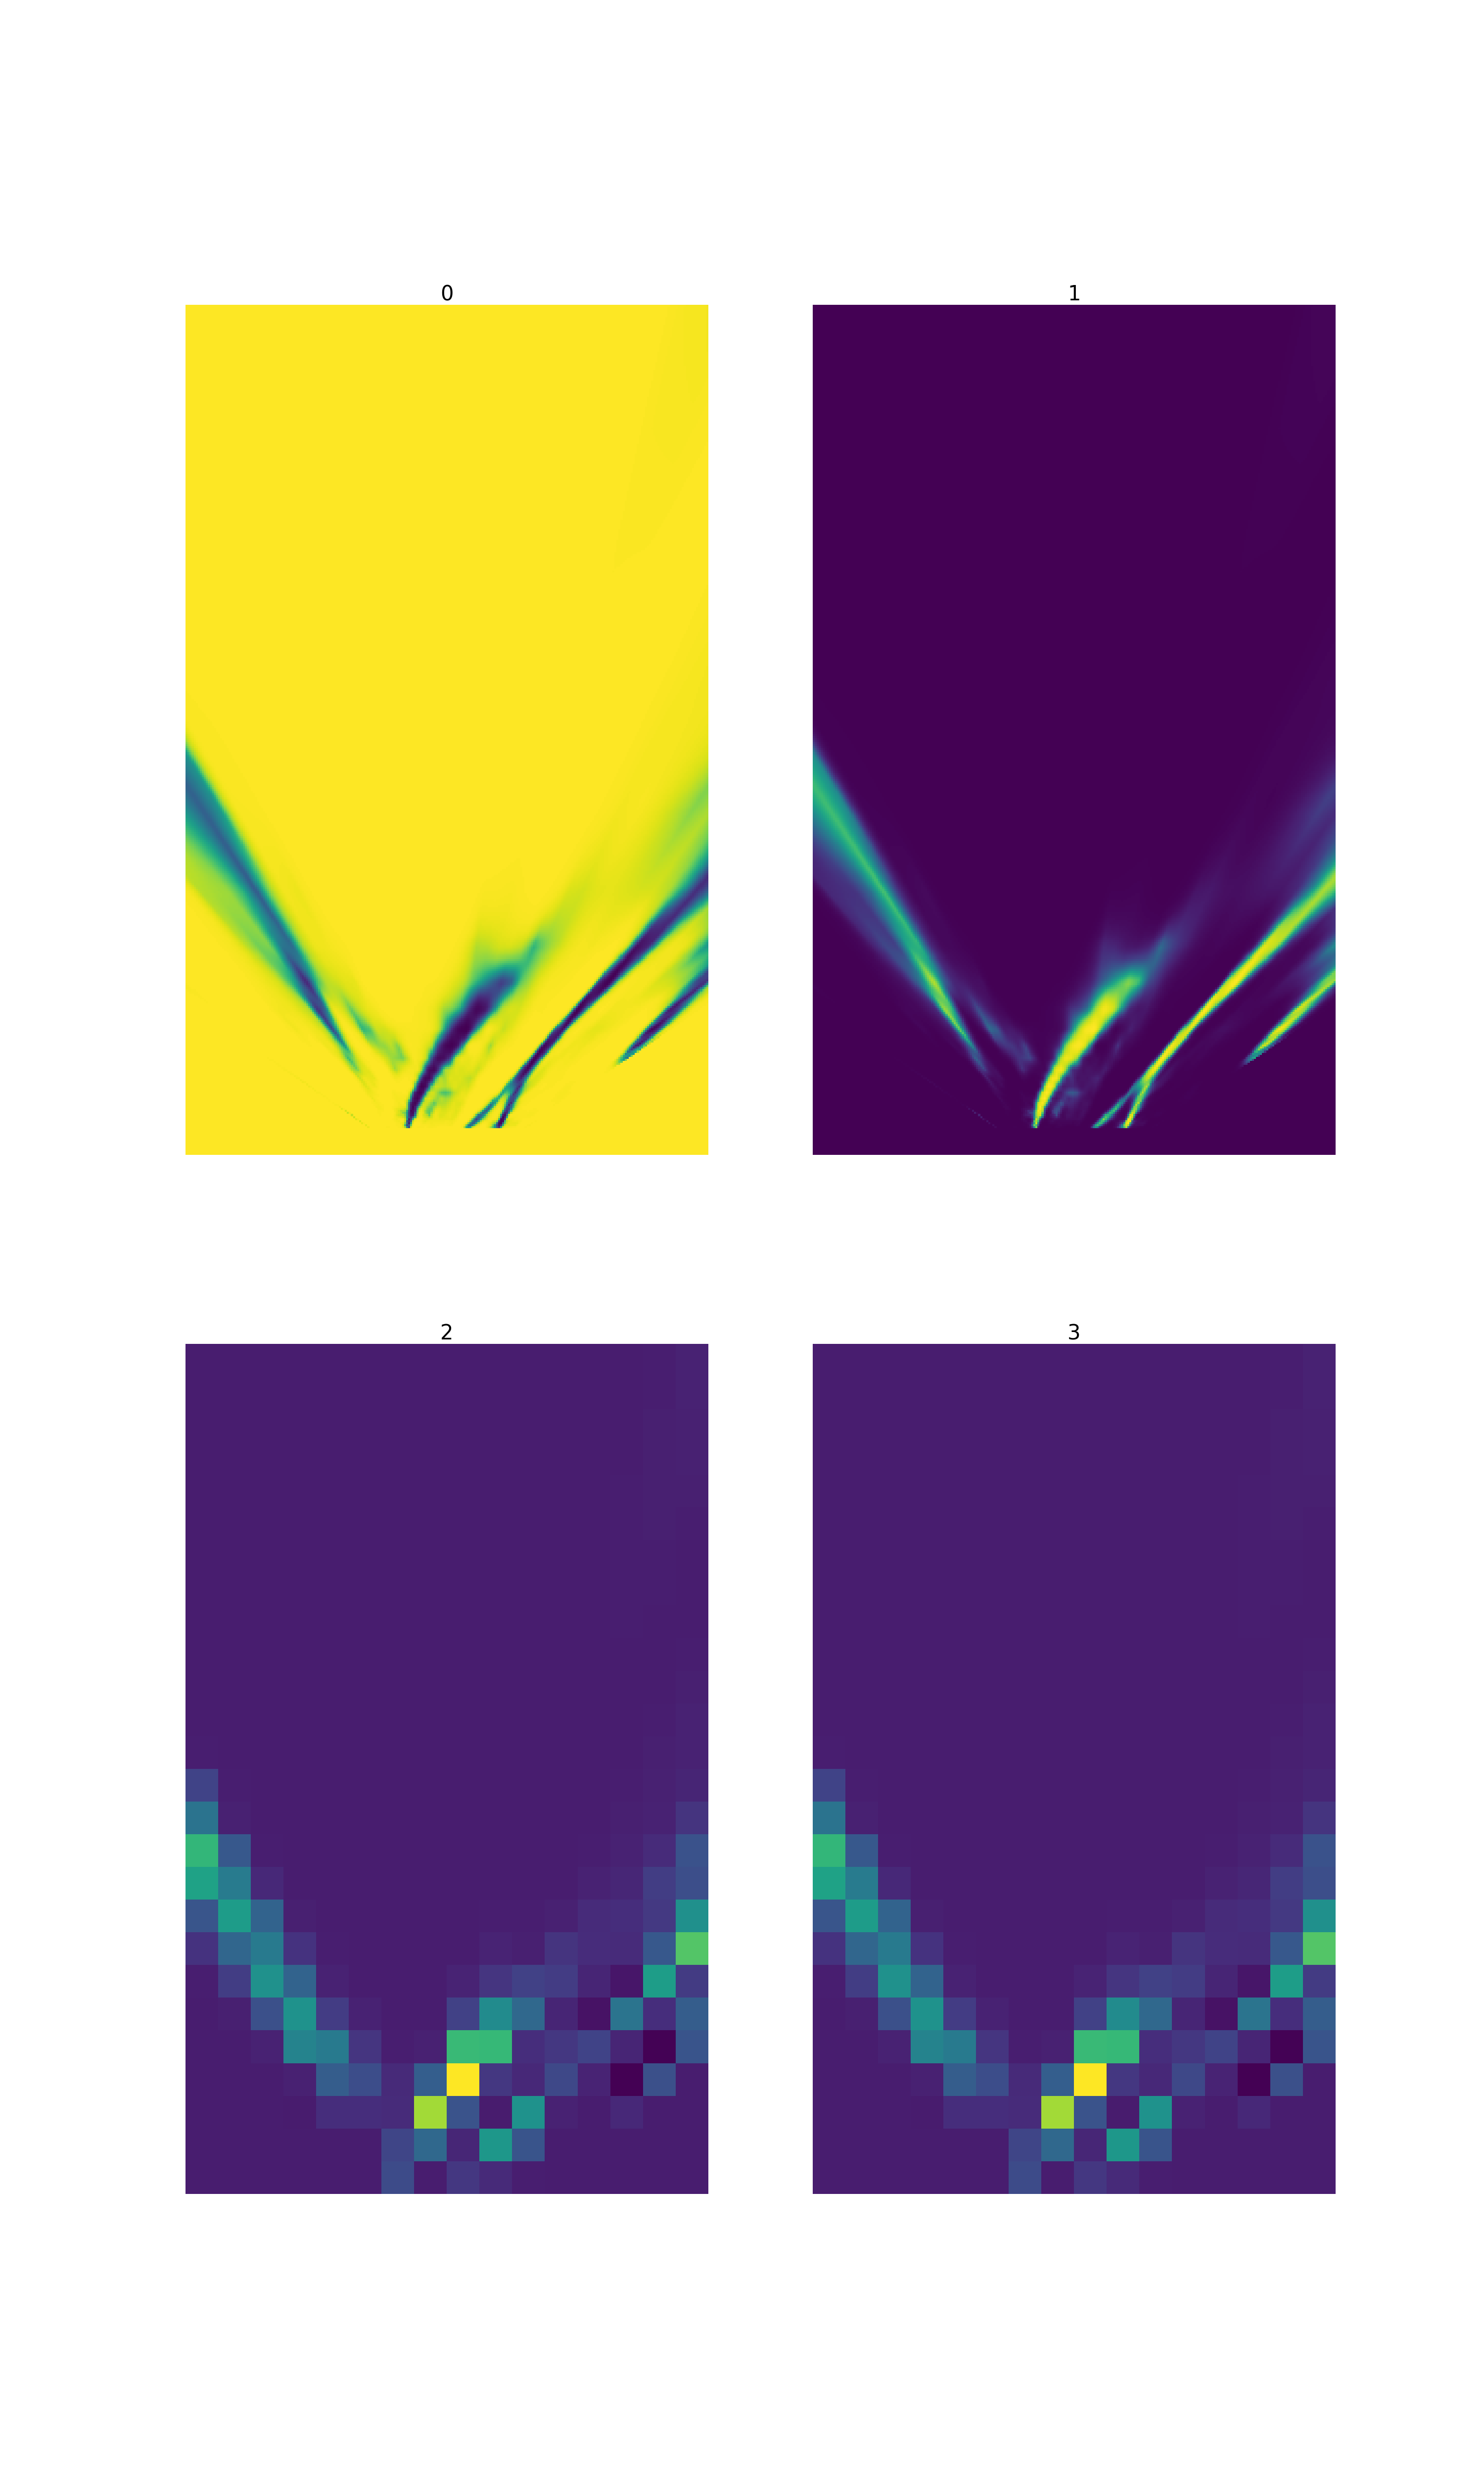
\includegraphics[width=1\linewidth,height=10cm]{images/embedding_regression_nofix.png}
        \caption{}
        \label{fig:subim2}
        \end{subfigure}
        \end{figure}

The regression pathway is responsible for regressing the lane geometric parameters like $r, \phi, \traingle z$ for each tile. Whereas the embedding pathway assign lane label to each tile to which it belongs to. The task of regressing geometric lane parameters is totally different from the task of learning embedding vectors for the lane curve clustering. We changed our approach by learning only one branch at a time. Which in return means that the loss from one branch is used to train the model for some initial epochs while keeping the parameters of the second branch frozen.  By using this schema we are able to train both pathways independently. 

 \begin{figure}[h]
      \caption{Activation maps of convolutional layers (a) embedding pathway (b) regression pathway, while training them independently}
        \centering
        \begin{subfigure}{0.8\textwidth}
        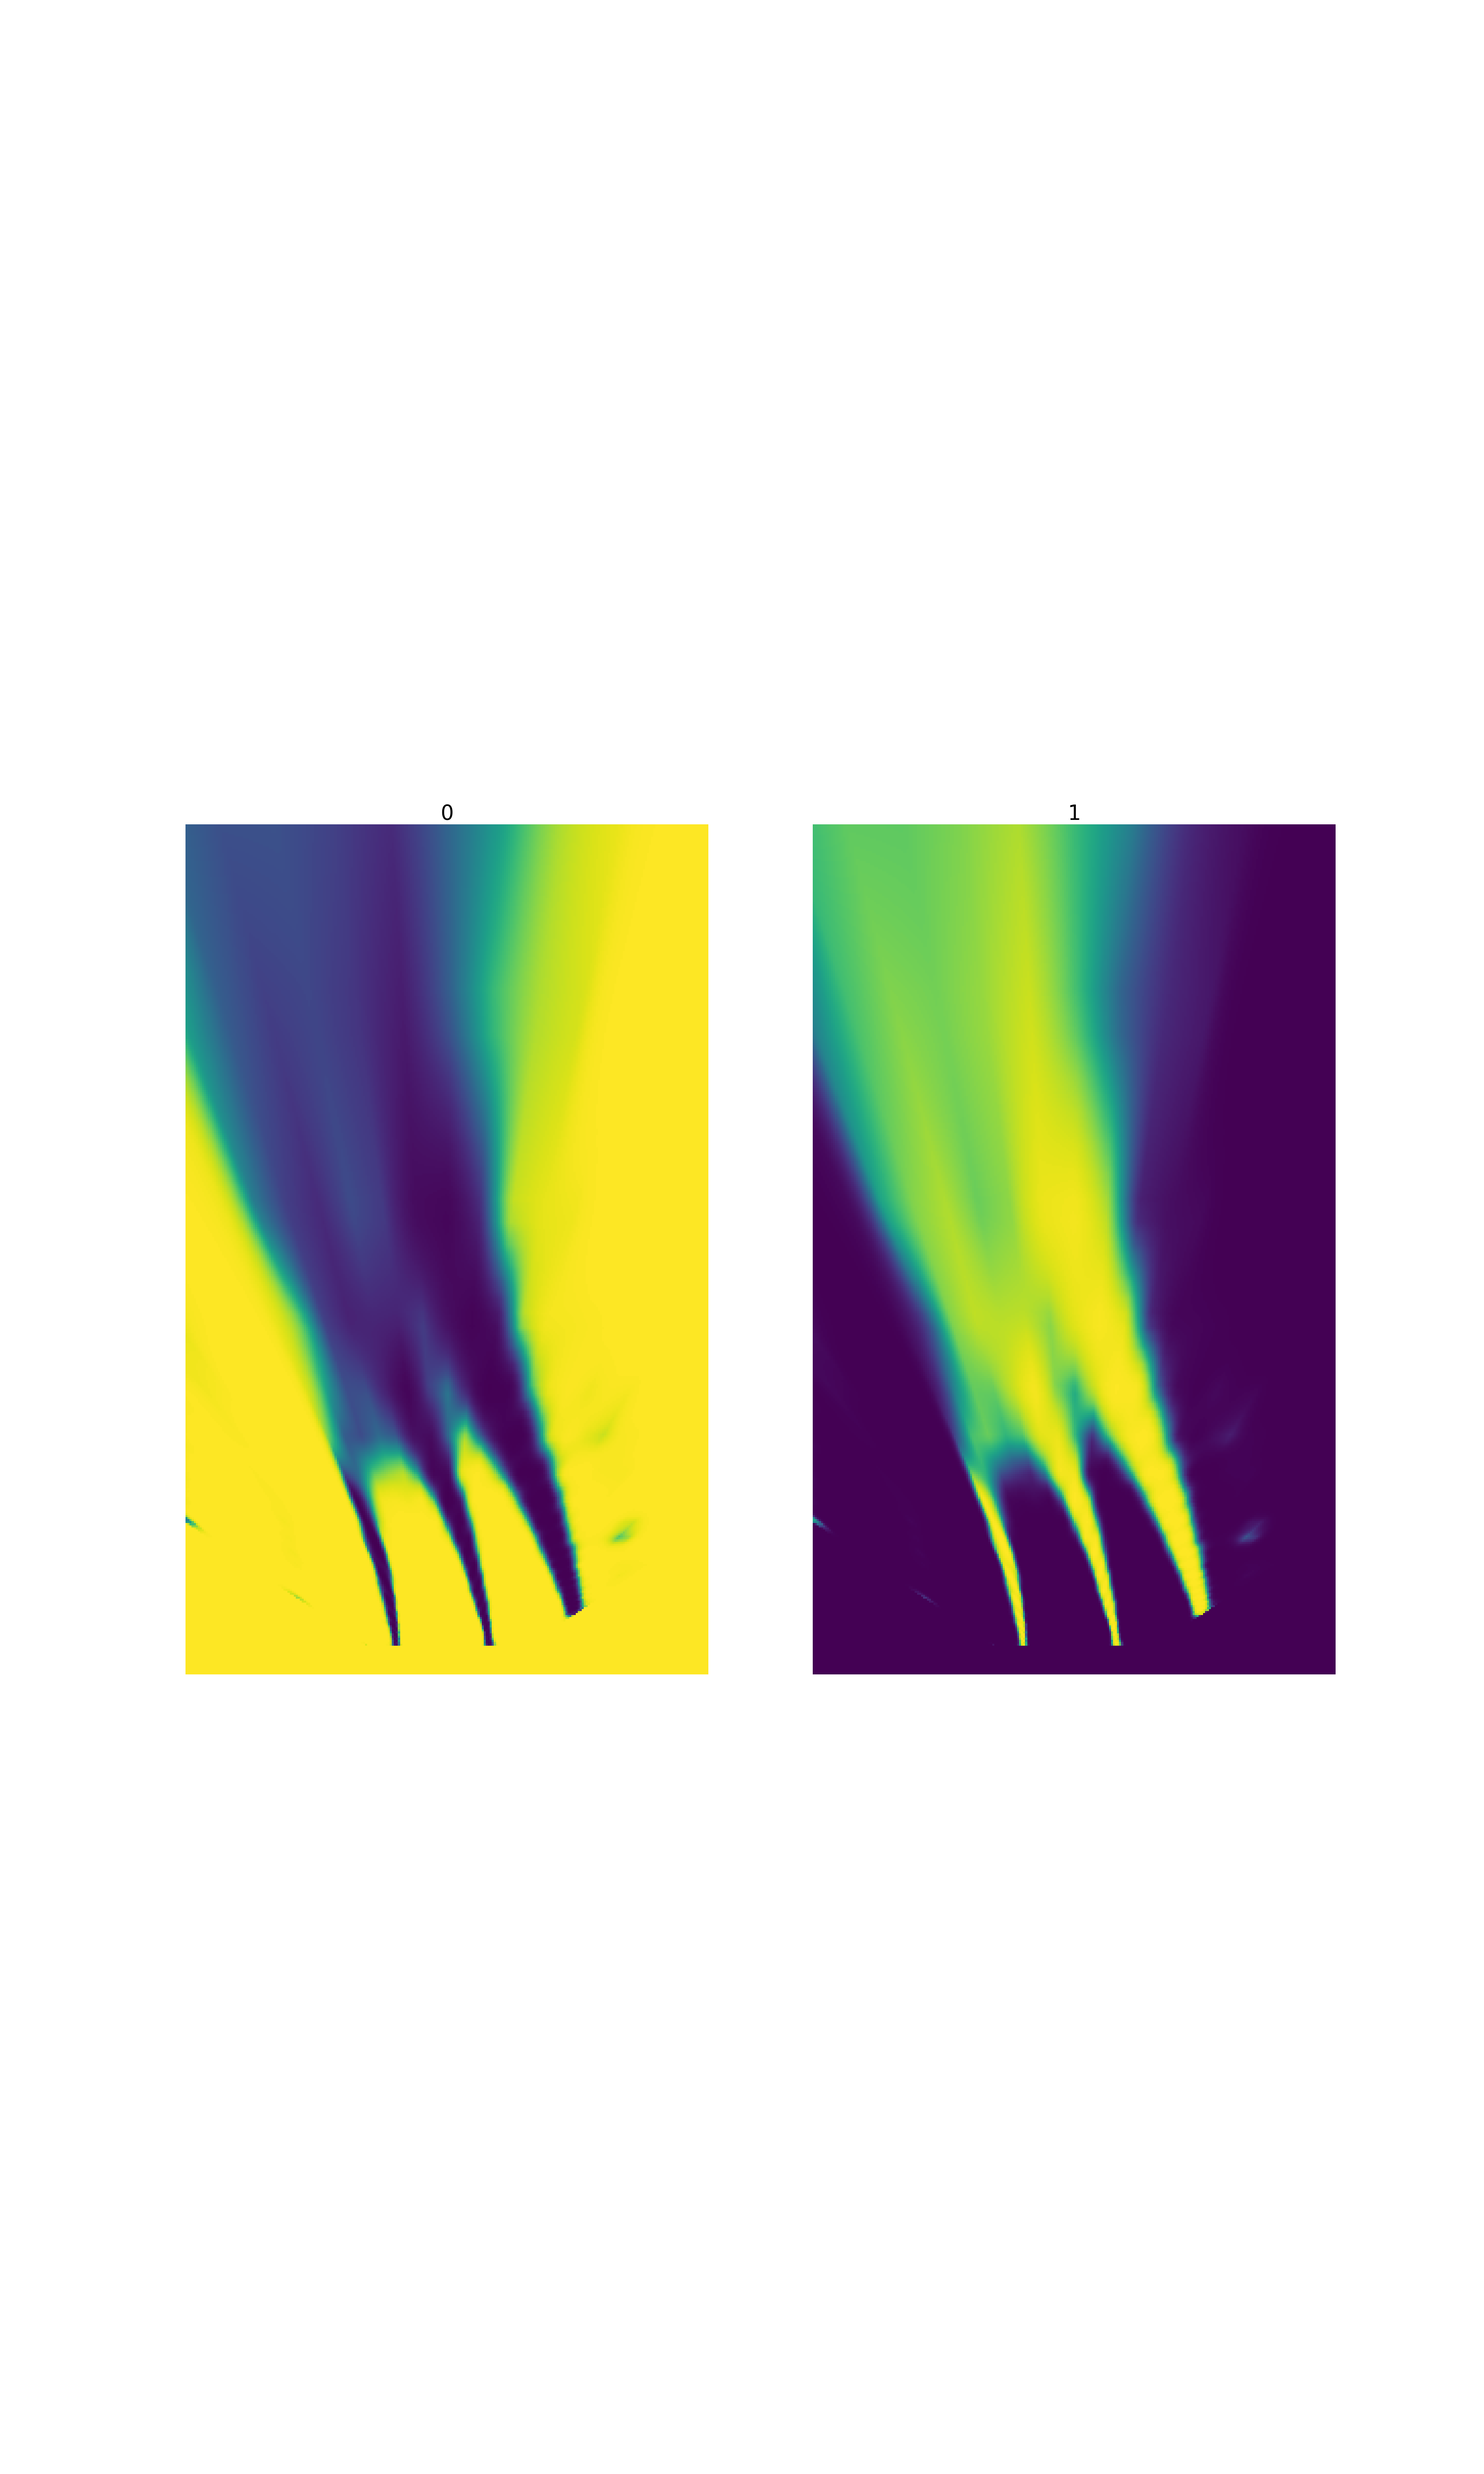
\includegraphics[width=1\linewidth, height=10cm]{images/activation_embedding.png} 
        \caption{}
        \label{fig:subim1}
        \end{subfigure}
        \begin{subfigure}{0.8\textwidth}
        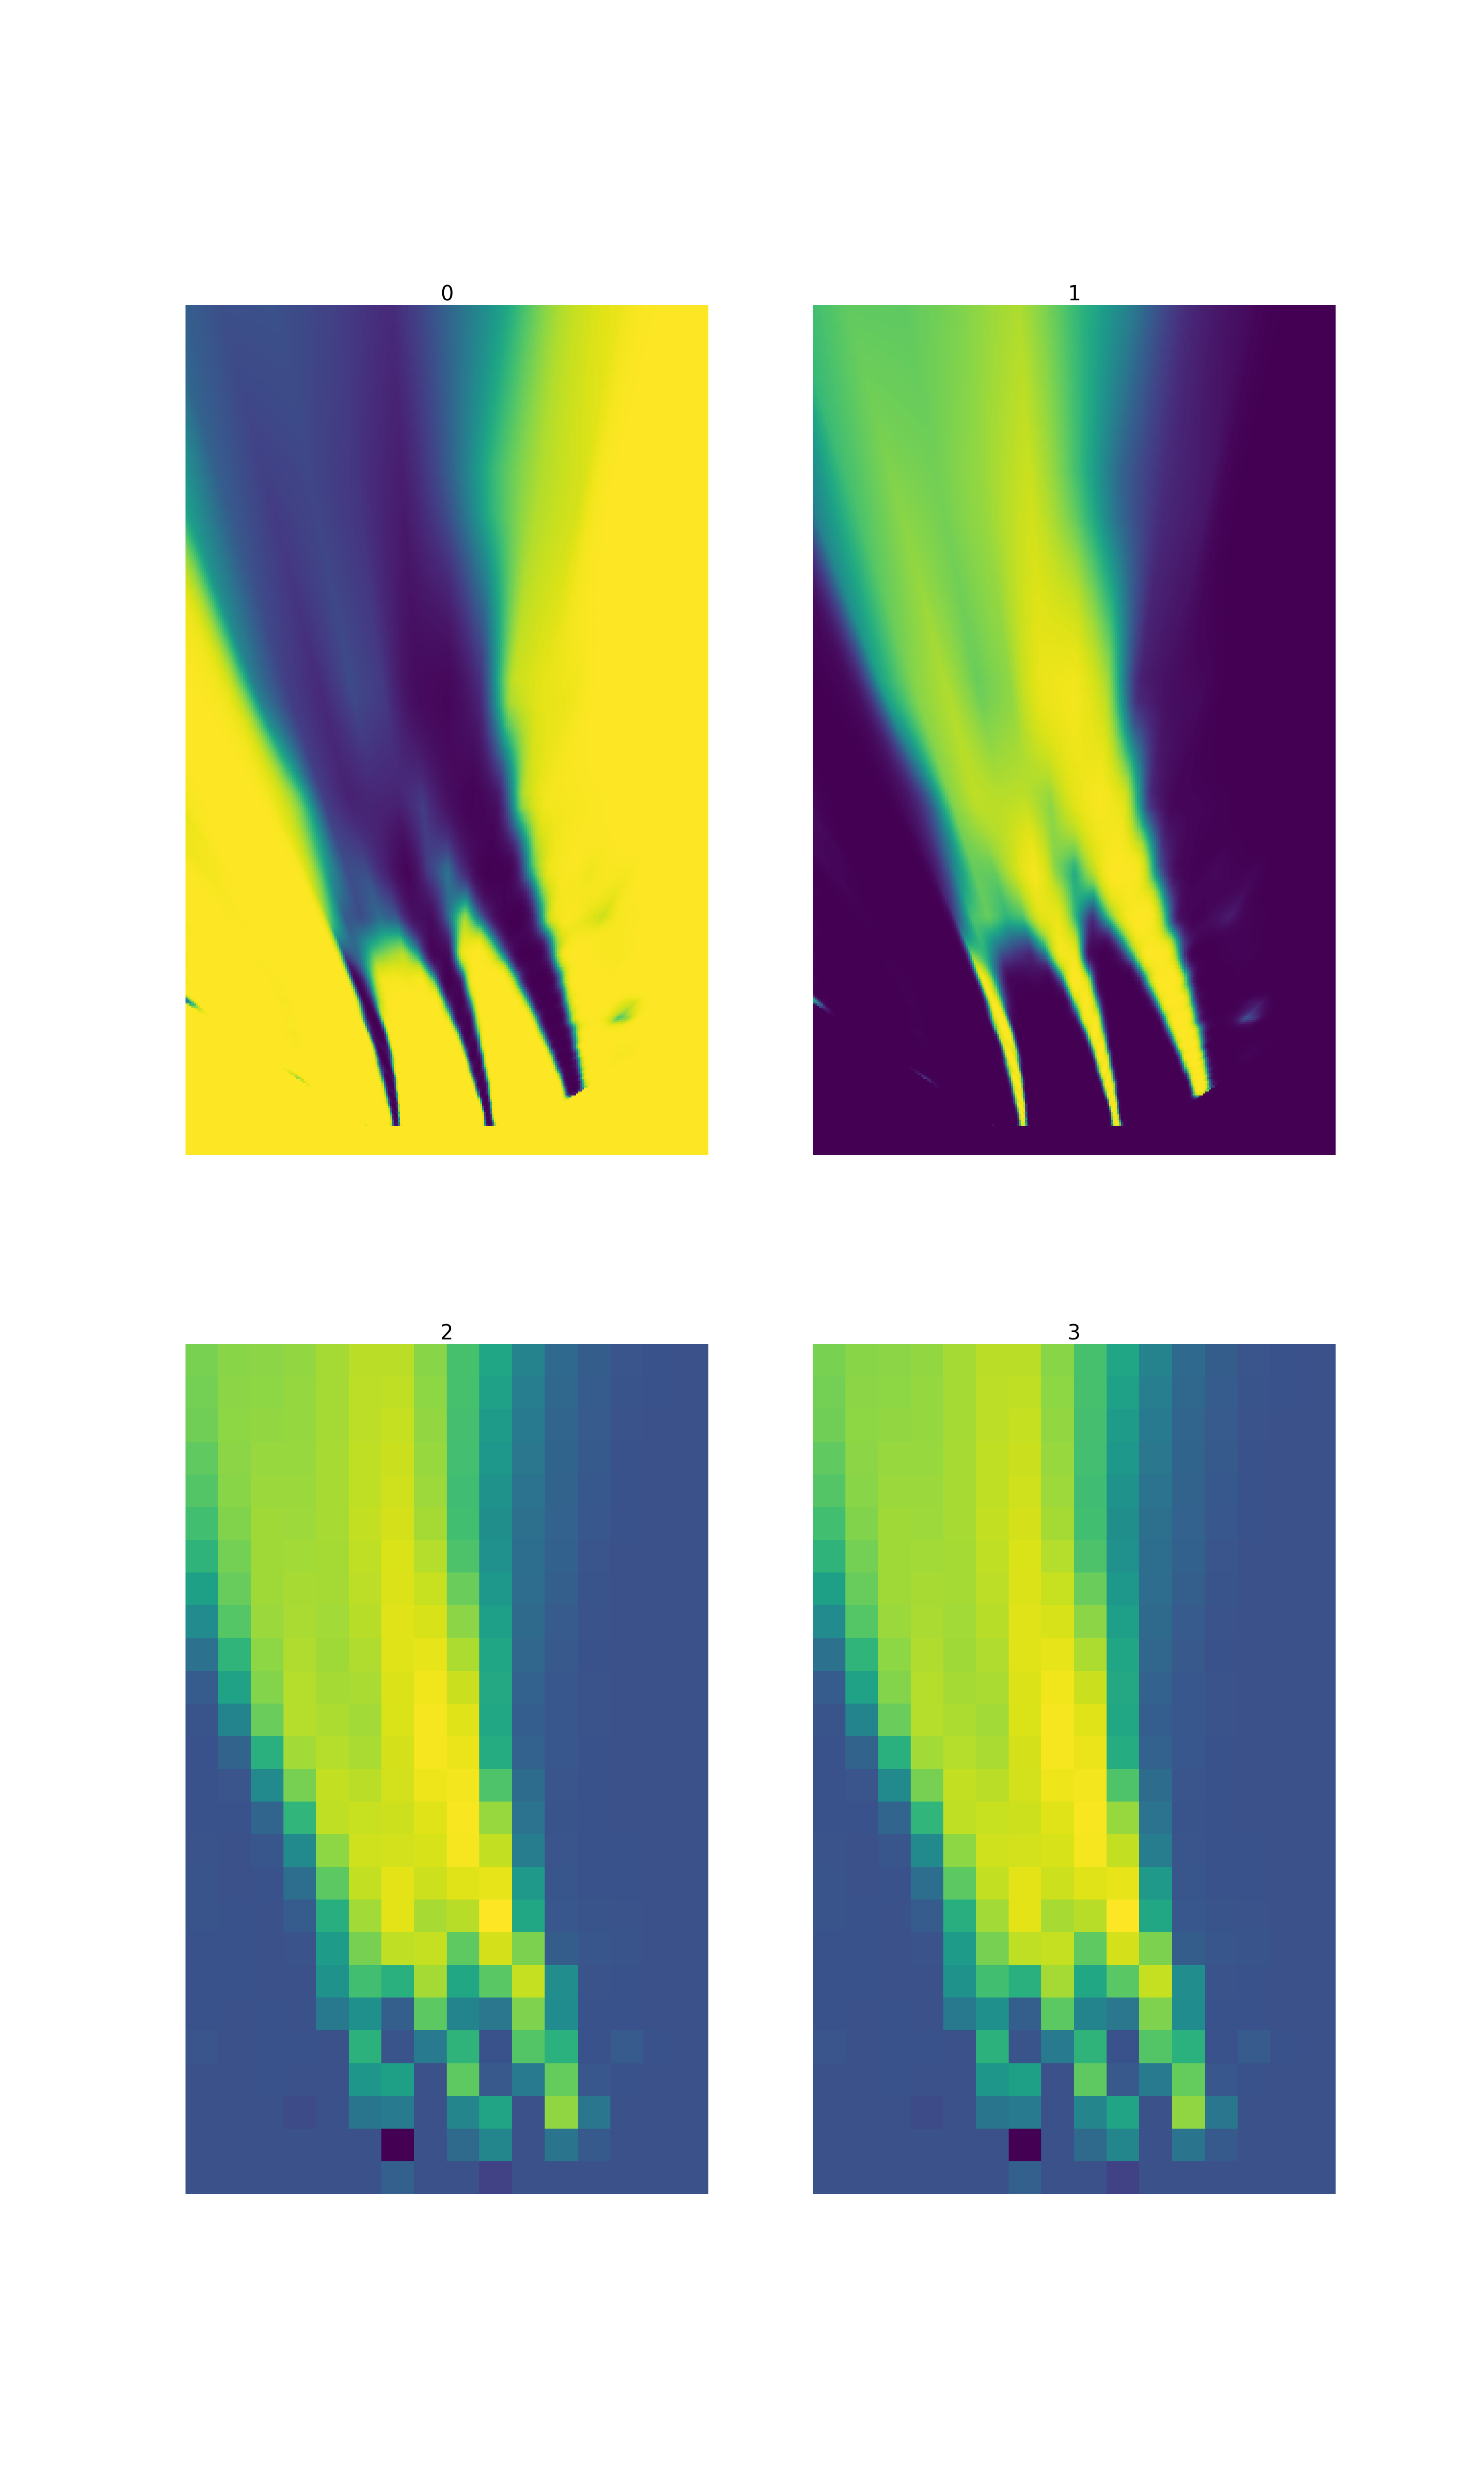
\includegraphics[width=1\linewidth,height=10cm]{images/activation_regression.png}
        \caption{}
        \label{fig:subim2}
        \end{subfigure}
        \end{figure}

Figure 5.10 validates our statement that by training both branches independently, the network is able to learn meaningful information from the input binary lane segmentation mask.

As we have discussed in section 4.2.5, $r_{i,j}$, $\phi_{ij}$ and $\triangle{z}_{ij}$ are regressed for each tile to approximate a 3D lane curve for that particular tile. Each tile contributes one point to the 3D lane curve. So it is really important to make sure that the regressed geometric lane parameters represent a 3D lane curve appropriately. After fixing the above-mentioned issue when the network is trained, we found that the geometric parameters regressed for 3D lane representation are not computed properly. To verify this statement we trace back the 3D lane curves from the ground-truth geometric parameters using equation 4.18 and found that they are incorrect. As per section 4.2.5, we have used the Hough Transform to approximate the lane segment which intersects each tile. To validate the correctness of the geometric parameters obtained via the Hough Transform, a single tile is processed via Hough Transform and the detected lane segment is visualized.

        \begin{figure}[h]
       \caption{Validating Hough Transform and visualizing the detected lane segment from a single tile}
        \centering
        \begin{subfigure}{0.8\textwidth}
        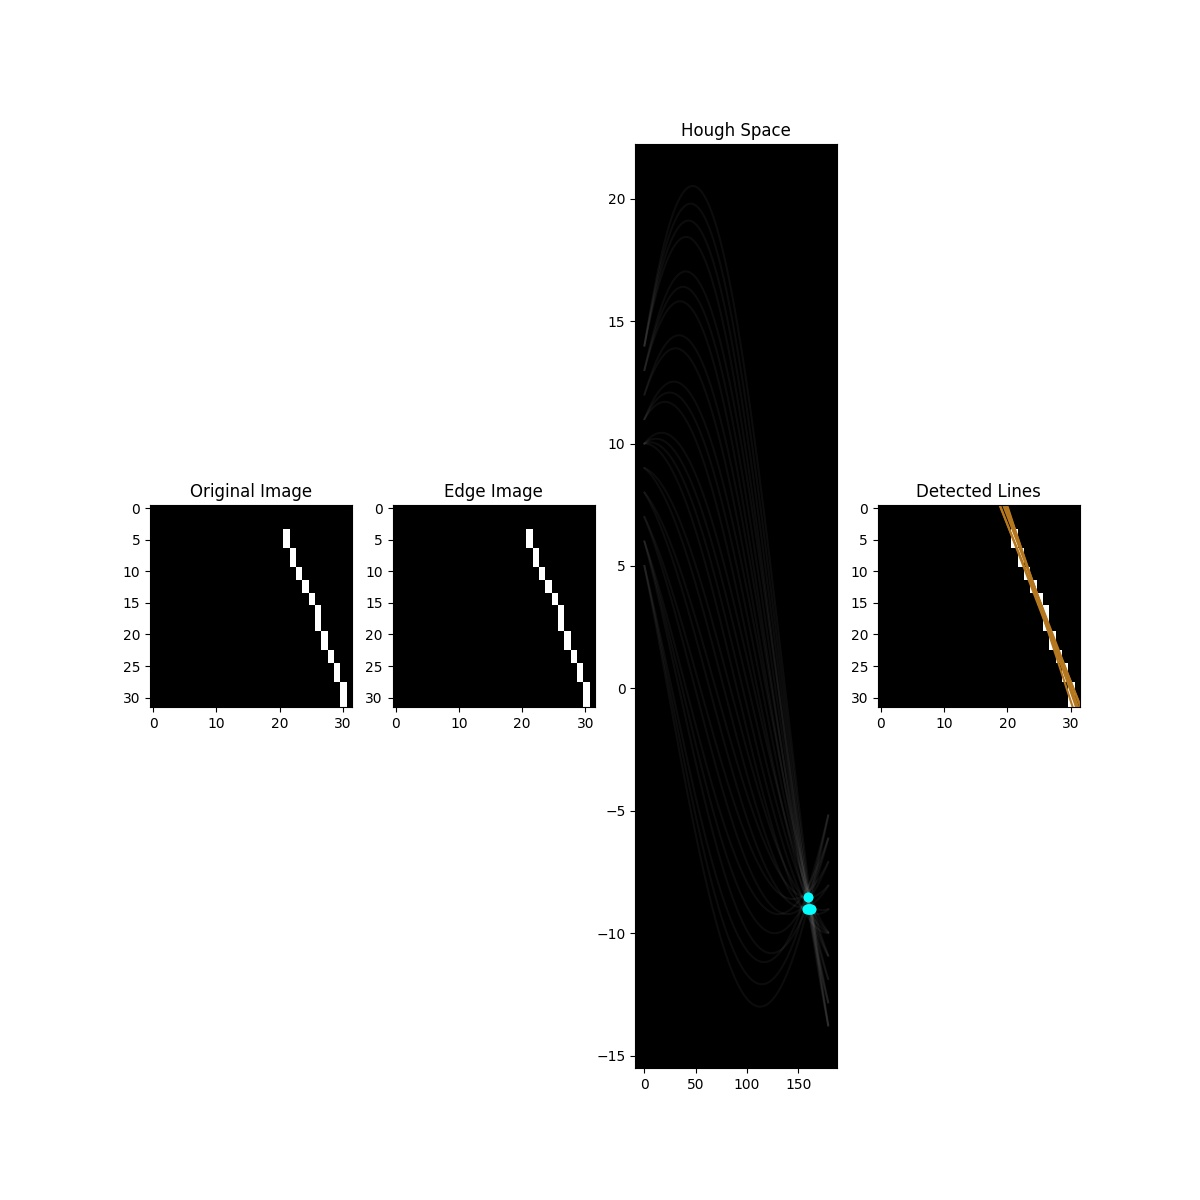
\includegraphics[width=1\linewidth, height=11cm]{images/hough_validation.jpg} 
        \label{fig:subim1}
        \end{subfigure}
        \end{figure}

Figure 5.11 shows the step-by-step process used to validate the Hough Transform. For each tile, When the geometric lane parameters obtained via Hough transform are transformed into 3D lane line points using equation 4.18. We observed that in the scenarios where the lanes are straight the x component of 3D points obtained after converting the polar to Cartesian coordinates were almost similar. Hough Transform is applied to each tile independently and the obtained geometric parameters are calculated with respect to the origin of each tile. Therefore the polar representation of the lane segment is in the vicinity of the tile itself. Therefore, we need to obtain $r_{i,j}$, $\phi_{ij}$ with respect to the global origin of the whole image. We utilized Hesse normal form and computed $r_{i,j}$, $\phi_{ij}$ for each tile with respect to the global origin of the image (top-left corner). Figure 5.12 and 5.13 validates that the obtained $r_{i,j}$, $\phi_{ij}$ for each tile is computed correctly. 


\begin{figure}[h]
      \caption{(a) Binary lane segmentation mask (b) Detected lanes via Hough Transform (c) Detected lanes via Hough Transform and using Hesse normal form as a post-processing step }
        \centering
        \begin{subfigure}{0.4\textwidth}
        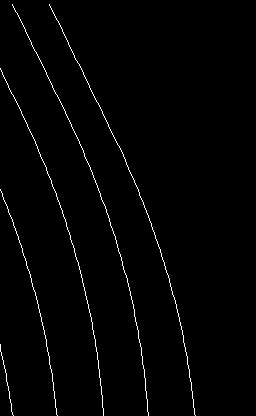
\includegraphics[width=1\linewidth, height=7cm]{images/test_bev_lanes.jpeg} 
        \caption{}
        \label{fig:subim1}
        \end{subfigure}
        \begin{subfigure}{0.4\textwidth}
        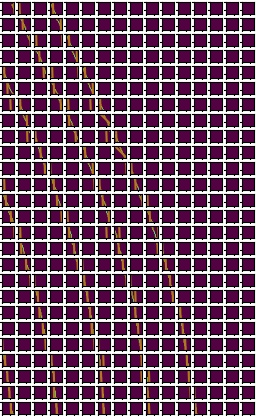
\includegraphics[width=1\linewidth,height=7cm]{images/detected_lines_r.jpg}
        \caption{}
        \label{fig:subim2}
        \end{subfigure}
        \begin{subfigure}{0.4\textwidth}
        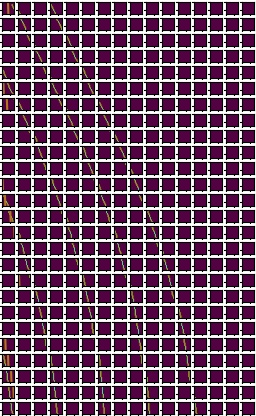
\includegraphics[width=1\linewidth,height=7cm]{images/detected_lines_rprime.jpg}
        \caption{}
        \label{fig:subim2}
        \end{subfigure}
        \end{figure}
        
Even after representing the geometric parameters obtained from each tile with respect to the global origin of the image, the obtained 3D lane curves are incorrect. To solve this issue we need to perform more debugging, which is unfortunately out of the scope of the defined duration of this thesis. Therefore we have added this to the list of future work, which we will talk about in more detail in the next section.
\end{document}
